\documentclass[11pt]{article}

% --- Packages ---
\usepackage[usenames, dvipsnames]{color} % Cool colors
\usepackage{enumerate, amsmath, amsthm, amssymb, mathrsfs, algorithm, algpseudocode, fontawesome, pifont, subfig, fullpage, csquotes, dashrule, tikz, bbm, booktabs, bm, hyperref}
\usepackage[framemethod=TikZ]{mdframed}
\usepackage[numbers]{natbib}
\usepackage[normalem]{ulem}

% --- Misc. ---
\hbadness=10000 % No "underfull hbox" messages.
\setlength{\parindent}{0pt} % Removes all indentation.

% -- Commands --
\input{commands}

\title{IEEE BigData 2019 Notes \\ \Large{Los Angeles, CA, USA}}
\author{Wenhao Zhang\footnote{\durl{http://wenhaoz.io}} \\ \durl{wenhaoz@ucla.edu}}
\date{Dec 2019}

\begin{document}
\maketitle
\tableofcontents
\newpage



\section{Conference Highlights}
\begin{figure}[ht!]
    \centering
    \includegraphics[width=140mm]{images/wordcloud.png}
    \caption{Trending research keywords in IEEE BigData 2019}
    \label{fig:my_label}
\end{figure}{}

This is the summary of conference highlights and my take-aways:

\begin{itemize}
    \item One quick take-away from this conference is that we can use ensemble learning combining different classifiers for FPG data analysis and Cardinal data analysis
    \item Federated learning is a very good research topic and there are many low hanging fruit. It's very useful in medical data analysis. Mayo clinic is also on this research topic. See section \ref{section: keynote1} for more info.
    \item The poster session is good, see section \ref{section:poster}
    \item Google has proposed a good dataset repo, {\bf DataCommons}, which I think is a better alternative to UCI machine learning repo. See section \ref{section:datacommmons}
    \item One paper talking about temporal causality, granger causality on Monday, interesting paper.
    \item Multi-task learning is gaining a lot of attention in medical + deep learning research.
    \item There are papers researching on EEG-based classification of Parkinson's disease
    \item This year, IEEE BigData conference has a lot of paper on deep learning.
    \item Wait for the conference proceedings coming out and we can read more details in the papers we are interested in.
    \item Potential Internship with Mayo Clinic and Potential collaboration with Mayo Clinic (Andrew Wen)

    
\end{itemize}{}



% \dblockquote{test}

% \todo{teset}

% \dnote{note}

% ------------
% -- Monday --
% ------------
\newpage
\section{Monday Dec 9th, 2019: Main Conference}
The conference begins! The first day is mostly workshop events.

\subsection{Workshop: Machine learning on Big Data}

\subsubsection{Transpose-based integrated data reduction techinques for speeding up classifier training}

{\bf Point 1:} Use feature selection methods (e.g., CFS, INFOGAIN, CHI-SQUARE) to select instance by transpose the matrix.\\

\remark{ The idea in this paper does not make sense to me. What if you have a small feature space and large instance sample size, i.e., $\mathbb{R}^{M \times N}$, where $M$ is large, and $N$ is small. The transpose matrix will be $\mathbb{R}^{N \times M}$ and your training sample will be insufficient for learning the parameters.}

\subsubsection{Reconstruction of agents' corrupted trajectories collective motion using low-rank matrix completion}

\ddef{Collective motion}{the collective motion trajectories of n agents. e.g., sheep usually travel in group}

Missingness might be observed in the trajectory matrix. Author use low-rank matrix completion to deal with the missingness. He also proves that collective motion is low rank.\\

$\ra$ Essentially this is a data imputation problem and can be approached using matrix factorization. \\

$\ra$ Authors haven't identify a real-world application yet. \\

\subsubsection{RecCite: A Hybrid Approach Recommend Potential Papers}

This paper uses all meta-data (e.g., age of publication) of a paper and citation relations to recommend to users.\\

Paper uses community detection to form clusters of users who are more related to each other (e.g., math community, computer science community, etc.). This greatly reduce the search space, hence scalability. 

\subsubsection{Parallel gradient boosting based granger causality learning}

\ddef{Granger causality}{Find the cause-effect relations in time series data}

Here is a tutorial on how to do a granger causality test: \url{https://www.statisticshowto.datasciencecentral.com/granger-causality/}\\

\note{This might be something related to temporal causality since granger causality test mines causal relations in time series data.}

\spacerule

\subsection{Workshop on Big Data Analytic Technology for Bioinformatics and Health Informatics}

\subsubsection{Explainable Deep Learning Applied to Understanding Opioid Use Disorder and Its Risk Factors}

\begin{itemize}
    \item Opiod Use Disorder (OUD) in veterans 
    \item logistic regression assumes independence among variables whereas DL doesn't have this issue.
\end{itemize}{}

\ddef{Impact assessment}{Calculate the feature importance used in the deep learning models}

The goal of this study is to develop a DL model for OUD prediction.

\begin{itemize}
    \item ReLU, Adam optimizer, 7 layers. 0.009 dropout
    \item 4\% OUD diagnosis (outcome).
    \item AUC comparison: DL:0.87, Logistic regression: 0.72
\end{itemize}{}

$\ra$ Impact scores in deep learning is comparable to correlation in conventional ways.

\subsubsection{Towards Explainable Melanoma Diagnosis: Prediction of Clinical Indicators Using semi-supervised and multi-task learning}

\ddef{Melanoma}{the most aggressive form of skin cancer}

The issue with melanoma is that the diagnosis is subjective and difficult.\\

This paper uses two dataset, e.g,  Indicator-dataset (226 samples) and Melanoma/Nevus datasets (9124 samples). This is where the multi-task learning can help. Since the two task of indicator-dataset and melanoma/nevus share some commonality, the model trained using Melanoma can help the model using Indicator-dataset. 

\idea{how can we incorporate multi-task learning in our breast cancer}

\subsubsection{Computer-Aided Clinical Skin Disease Diagnosis Using CNN and Object Detection Models}

skin disease diagnosis in certain areas is expensive and usually is not accessible. So machine learning/deep learning can help in detecting skin diseases.\\

Use existing DL classifiers to test on their dataset and develop their own DL model: They tested 4 different DL models and later ensemble them as a new DL model.\\

\note{Object detection/region of interest can help diagnosis since certain ROI are relatively small in the images. With the ROIs labeled, we focus our classification only on the interested region.}\\

$\ra$ Ensemble strategy: linear summation (avg. predict\_prob?).

\idea{for the cardinal dataset/FPG dataset, can we use ensemble strategy with multiple classifiers?}

\subsubsection{Automated Machine Learning for EEG-Based Classification of Parkinson's Disease Patients}

$\ra$ Identify the high/poor cognition

$\ra$ Feature selection algo: Boruta algorithm \cite{kursa2010feature}

\subsubsection{Recurrent Neural Network Based Feature selection for High Dimensional and Low Sample size Micro-array Data}

{\bf Issue}
\begin{itemize}
    \item Data sparsity, many 0s in the matrix
    \item High dimension, but only small portion of features correlate with target.
\end{itemize}

$\ra$ Inspired by paper \cite{liu2017deep}, the proposed method extends to recurrent neural network.

\subsubsection{Baysian Non-linear Support Vector Machine for High-dimensional Data}

\mov{Current SVMs assume 1) linear separation, 2) independence between features, which are usually not true in medical settings.}\\

$\ra$ contribution: 1) incorporate knowledge graph into the prior distribution in beysian inference. 2) more interpretable path analysis from the knowledge graph.\\

$\ra$ graphs converts into adjacency matrix, which is easier to be incorporated into the prediction model.\\

\subsubsection{Predicting Post-stroke Hospital Discharge Disposition Using Interpretable Machine Learning Approaches}

$\ra$ de-mythologize the black-box of machine learnings.

$\ra$ Data: 130,000 data samples with ICD9 code.

$\ra$ The proposed method, LIME, pick a subset of the dataset and try to change the value of the features and see how does the change affect the predictions. In Scikit-learn, feature selection is done using the whole dataset. But LIME uses only a small subset of it which is ``representative" of the whole population. In other words, the subset has the close degree of variety as the population.

\remark{This might be why the algorithm could be scalable in large dataset.}

\subsubsection{Exploiting Anti-Monotonic Constraint for Mining Palindromic Motifs from Big Genomic Data}

\mov{Existing methods such as dynamic programming for mining panlidromic motifs demands high computational resources (e.g., memory and time)}\\

$\ra$ proposed method handles with high volume of genomic data efficiently in parallel.\\

$\ra$ runs on Apache Spark\\

$\ra$ exploit anti-monotonic constraint: if a sub-sequence is not a palindromic mortifs (PM), then the super-sequence is not a PM.

\spacerule



% ------------
% -- Tuesday --
% ------------
\newpage
\section{Tuesday Dec 10th, 2019: Main Conference}
This is the second day! Presented our imbalanced learning work, and attended a few keynotes.

\subsection{Special session on intelligent data mining}

\subsubsection{Understanding Multilingual Communities through Analysis of Code-switching Behaviors in Social Media Discussions}

$\ra$ Research interests: twitter discuss with replies that are  multilingual. \\

$\ra$ To understand why people are changing languages in tweets replies.

datasets are human tagged, to identify whether a reply has a complete sentence in a language, and score the relevance of the reply.

\subsubsection{Explainable Visualization for interactive exploration of CNN on Wikipedia Vandal Detection}

Focused on explainable machine learning using visualization. Previous works that try to be white-box are on neuron-level which are not intuitive for layman.

\spacerule

\subsection{IEEE BigData Cup Challenge}

\subsubsection{Emotion detection using EEG signal with CNN}

Dataset: DEAP dataset, a public  dataset for emotion;\\

Classifier: SVM and CNN, interestingly, CNN is way worse  than SVM as there  are not  enough data for training a better CNN.\\

$\ra$ use  data augmentation to  increase  the  training dataset size by generating artificial data samples.\\

Data augmentation: add Gaussian noise (does not change amplitude data).\\

Data augmentation and  data  reshape has increased  the performance of  CNN tremendously, from nearly 0.65 to 0.96 (accuracy)\\

\begin{figure}[ht!]
    \centering
    \includegraphics[width=120mm]{images/eeg.png}
    \caption{EEG feature extraction}
    \label{fig:eeg}
\end{figure}

\spacerule

\subsection{Keynote 1: Federated Recommendation}

\label{section: keynote1}

The speaker is Qiang Yang who is from the WeBank and Hong Kong University of Science and Technology.\\

\note{In recommender system, the more data the better system. Through web crawling, business contract, we can have more data sources. But the question is "is this approach sustainable?"}

\note{In health care systems, ``federated learning" is pretty important as it protects the privacy of clinical data. This could be another research direction in the future and the speaker says there are a lot of low-hanging fruit in this research area}

Conventional machine learning requires centralizing the training data on one machine or in a data center. And Google has built one of the most secure and robust cloud infrastructures for processing this data to make our services better. Now for models trained from user interaction with mobile devices, we're introducing an additional approach: Federated Learning. 

\ddef{Federated learning}{Federated Learning is a machine learning setting where the goal is to train a high-quality centralized model with training data distributed over a large number of clients each with unreliable and relatively slow network connections.}

\ddef{data silos}{data islands that are shared between research entities as security issues or other reasons.}

$\ra$ The federated learning is good for protecting data privacy as the training process is decentralized.\\


{\bf FATE}\footnote{\url{https://github.com/FederatedAI/FATE}} is a open-source framework for industrial federated recommender system

\subsubsection{Keynote 2: the new science of cause and effect, with reflections on data science and artificial intelligence}

The speaker is Judea Pearl. 

{\bf Why data science needs a new engine, to answer causal questions.}\\

The seven tools of causal inference

\begin{itemize}
    \item Encode causal info in transparent and testable way.
    \item Predicting the effects of actions and policies.
    \item Computing counterfactuals and finding causes of effects
    \item Computing direct and indirect effects (Mediation)
    \item Integrating data from diverse sources
    \item Recovering from missing data
    \item Discovering causal relations from data (growing field)
\end{itemize}

\remark{Causal relation discovery is a growing field and we can check in the literature from CMU and UCLA on the related work.}

\remark{current science build on equality(y=ax equals to x = y/a), hence cannot answer uni-directional questions, e.g., causal questions}

\begin{figure}[htbp!]
    \centering
    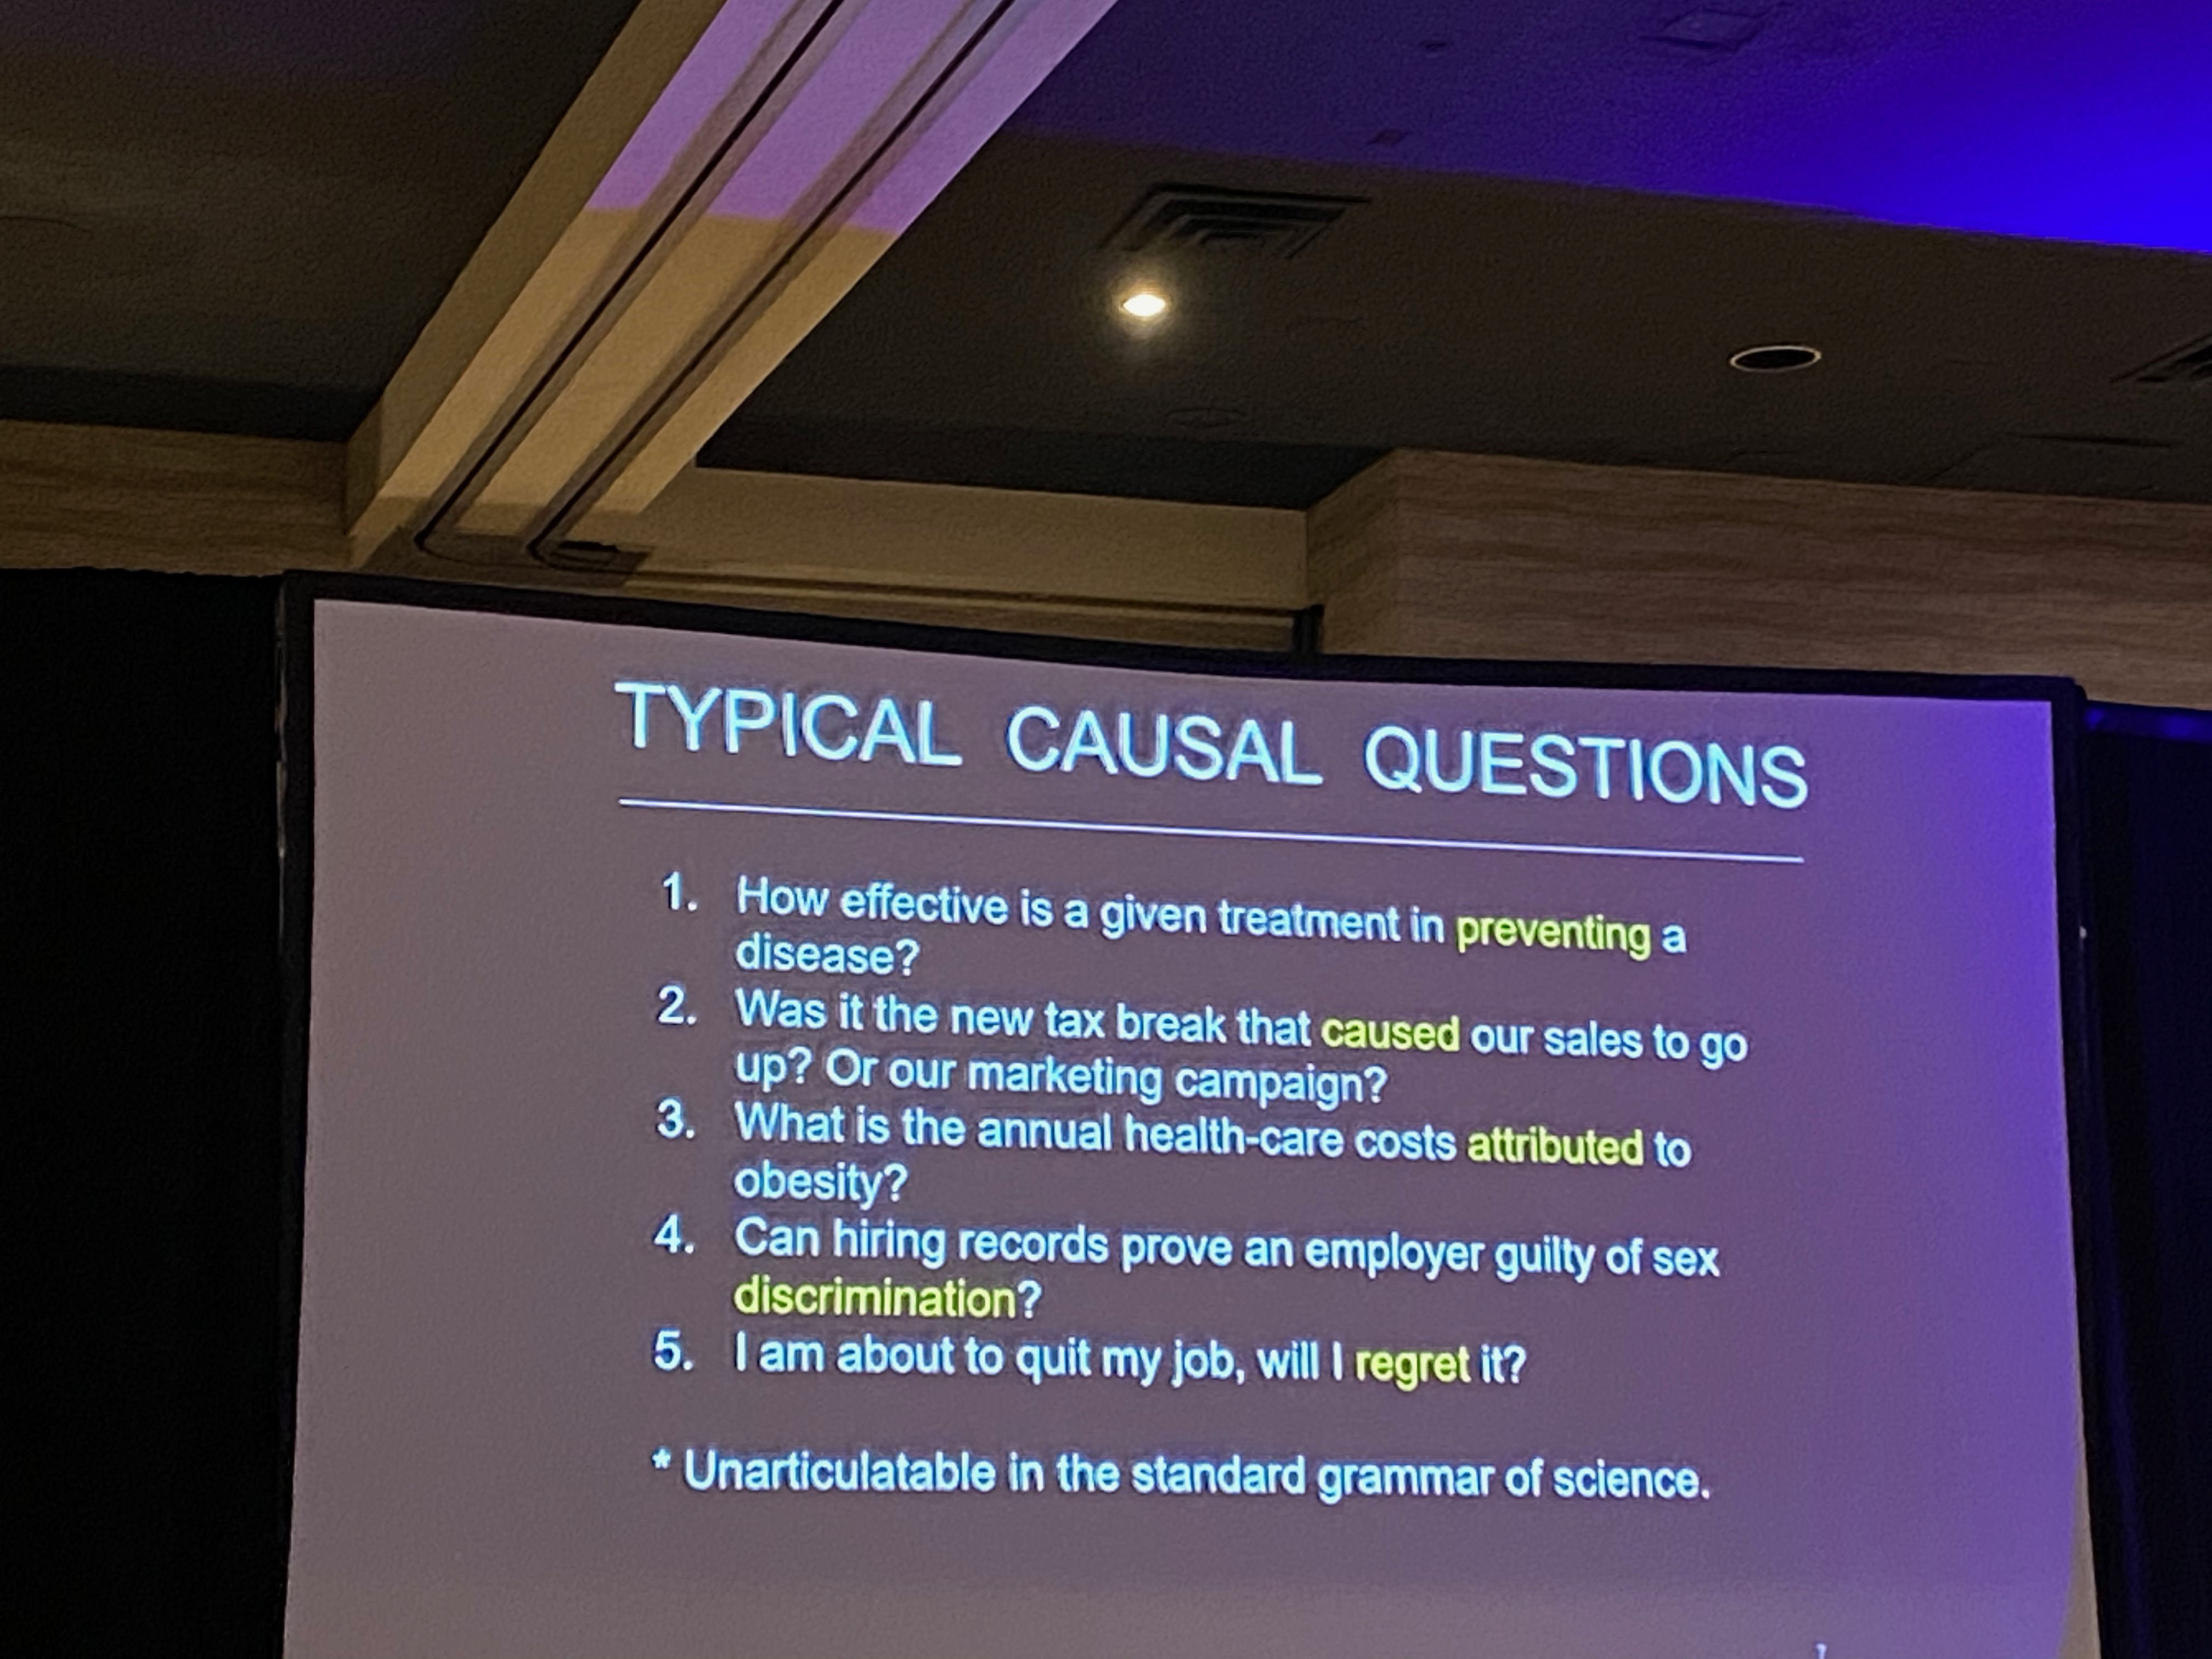
\includegraphics[width=120mm]{images/causal_questions.png}
    \caption{Causal questions}
    \label{fig:causal_questions}
\end{figure}

\begin{figure}[htbp!]
    \centering
    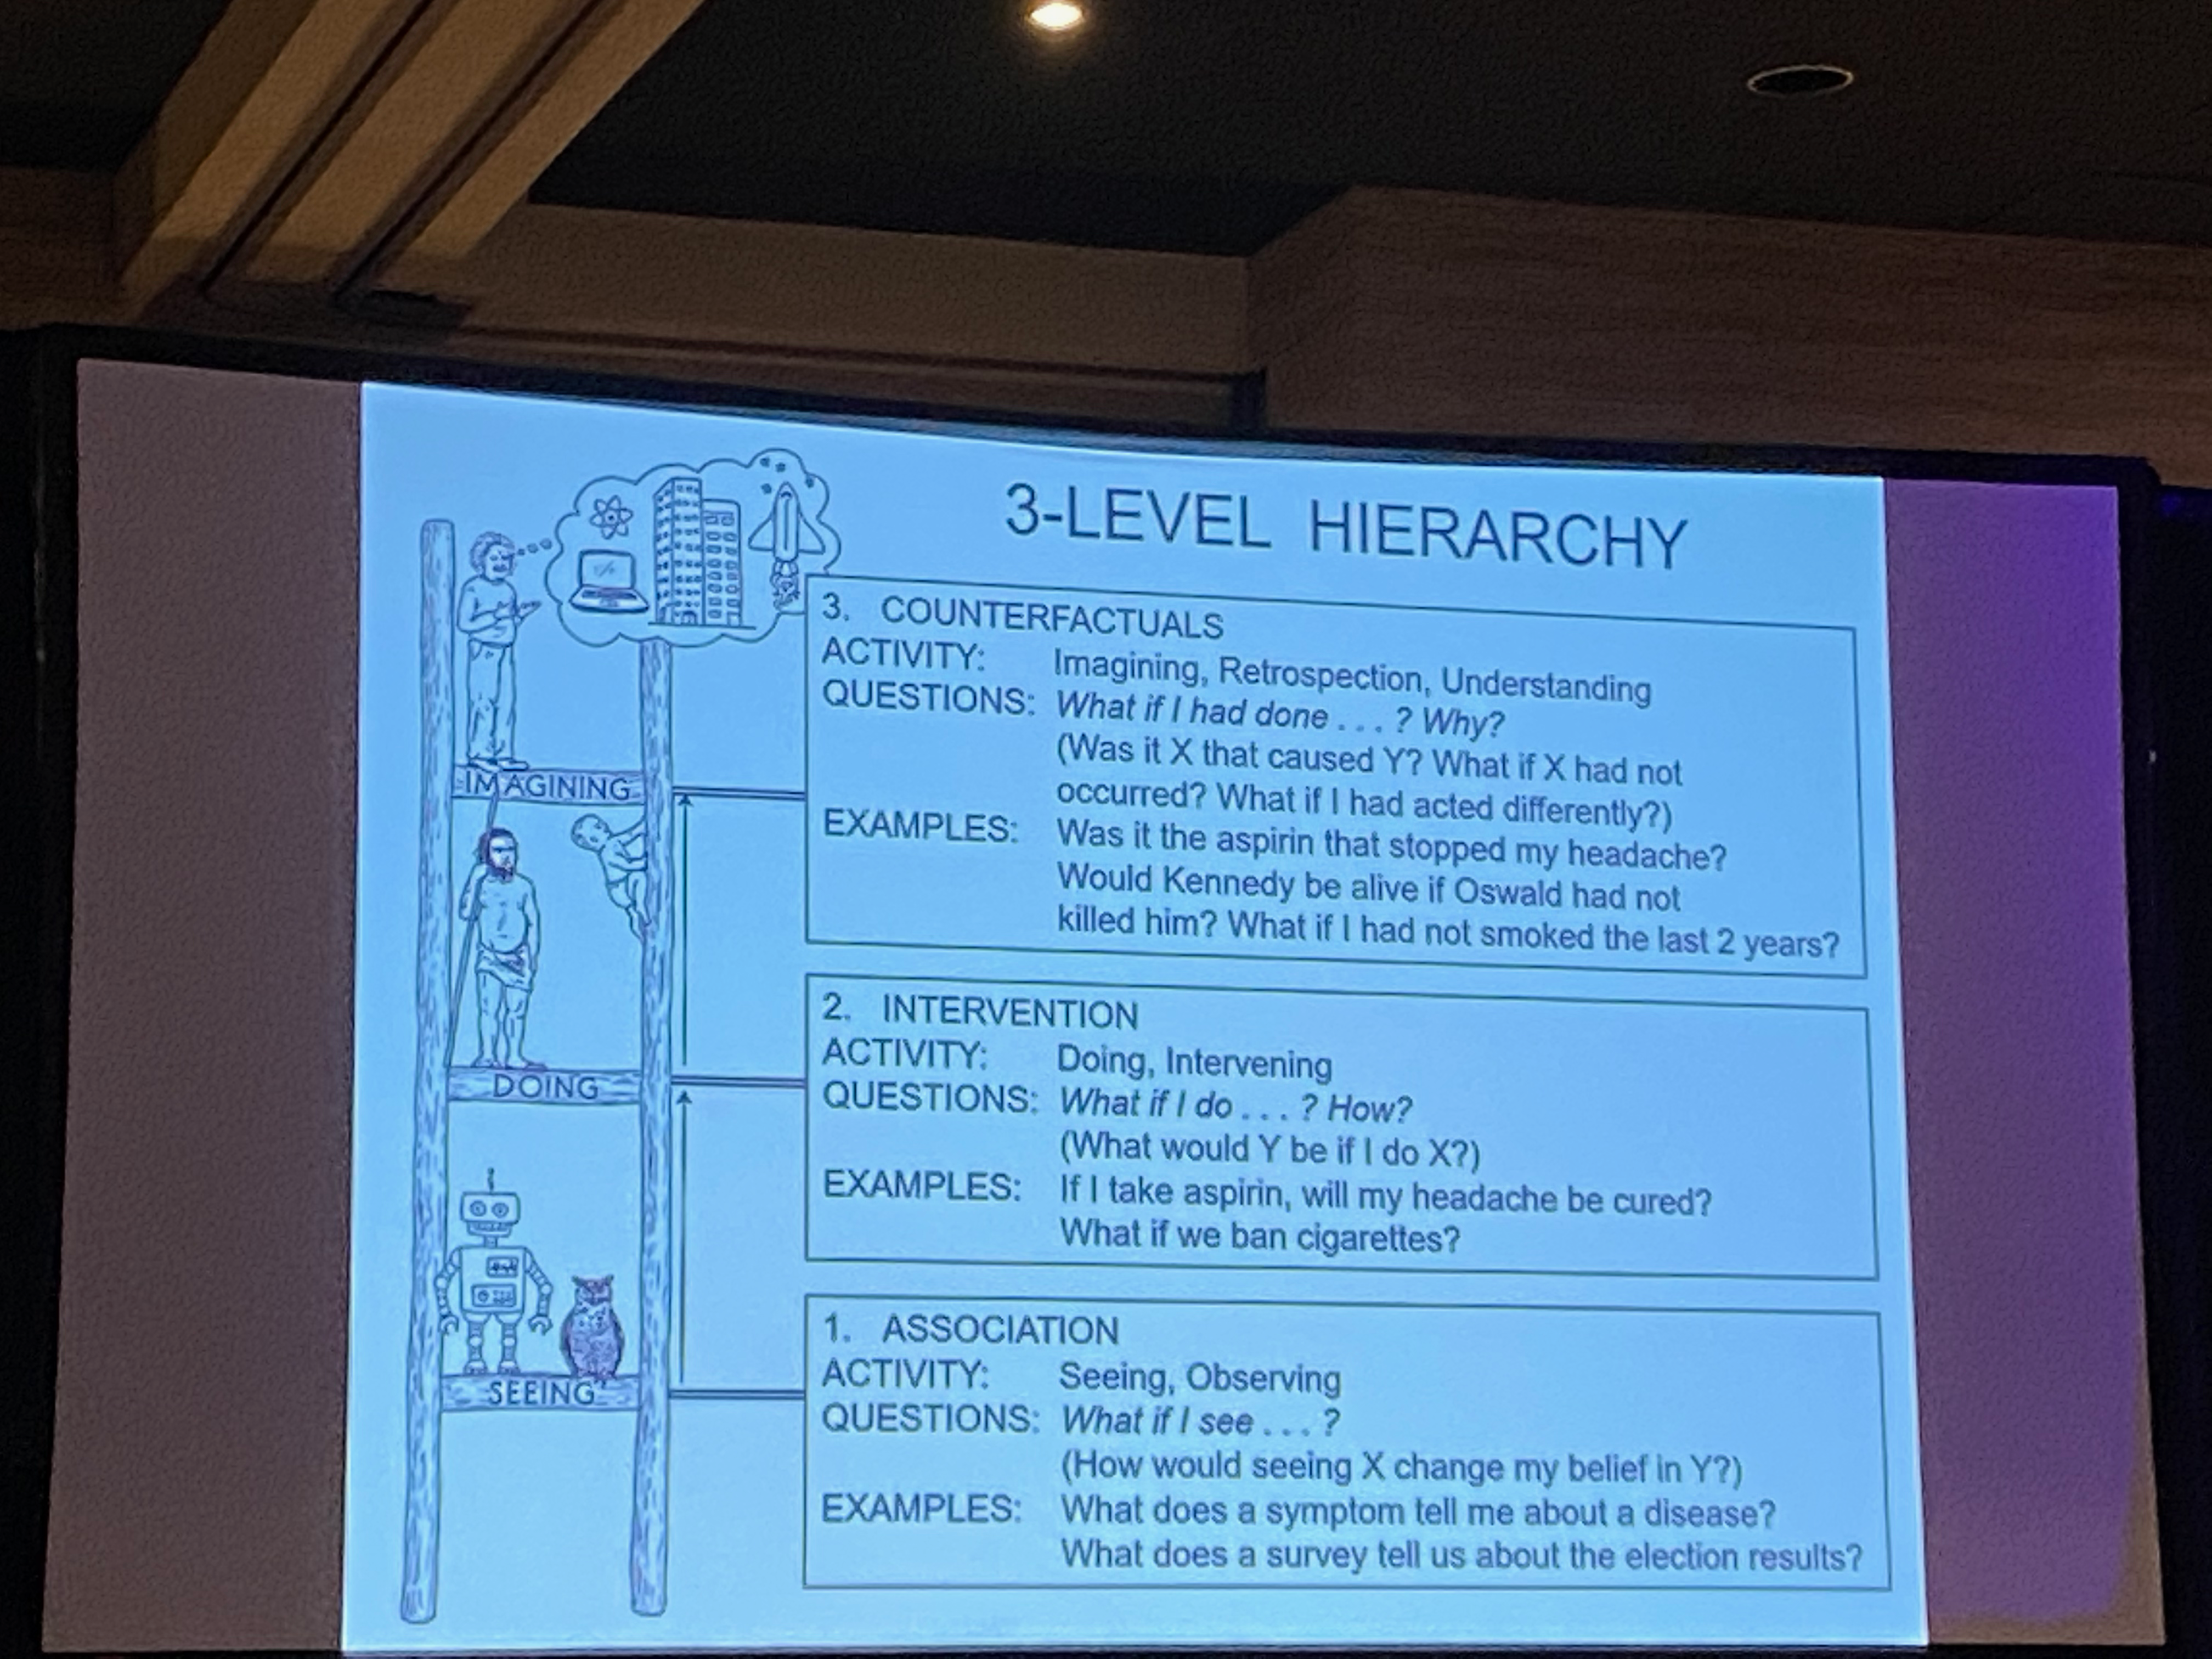
\includegraphics[width=120mm]{images/causal_ladder.png}
    \caption{3-level Causal ladder}
    \label{fig:causal_laddar}
\end{figure}

\idea{Can we answer the question: how much data missing is too much using Mohan and Pearl's work}



\spacerule

% ------------
% -- Wednesday --
% ------------
\newpage
\section{Wednesday Dec 11th, 2019: Main Conference}
This is the third day! Most of the regular paper presentation happen today.

\subsection{Poster display}
\label{section:poster}

\begin{figure}[!ht]
    \centering
    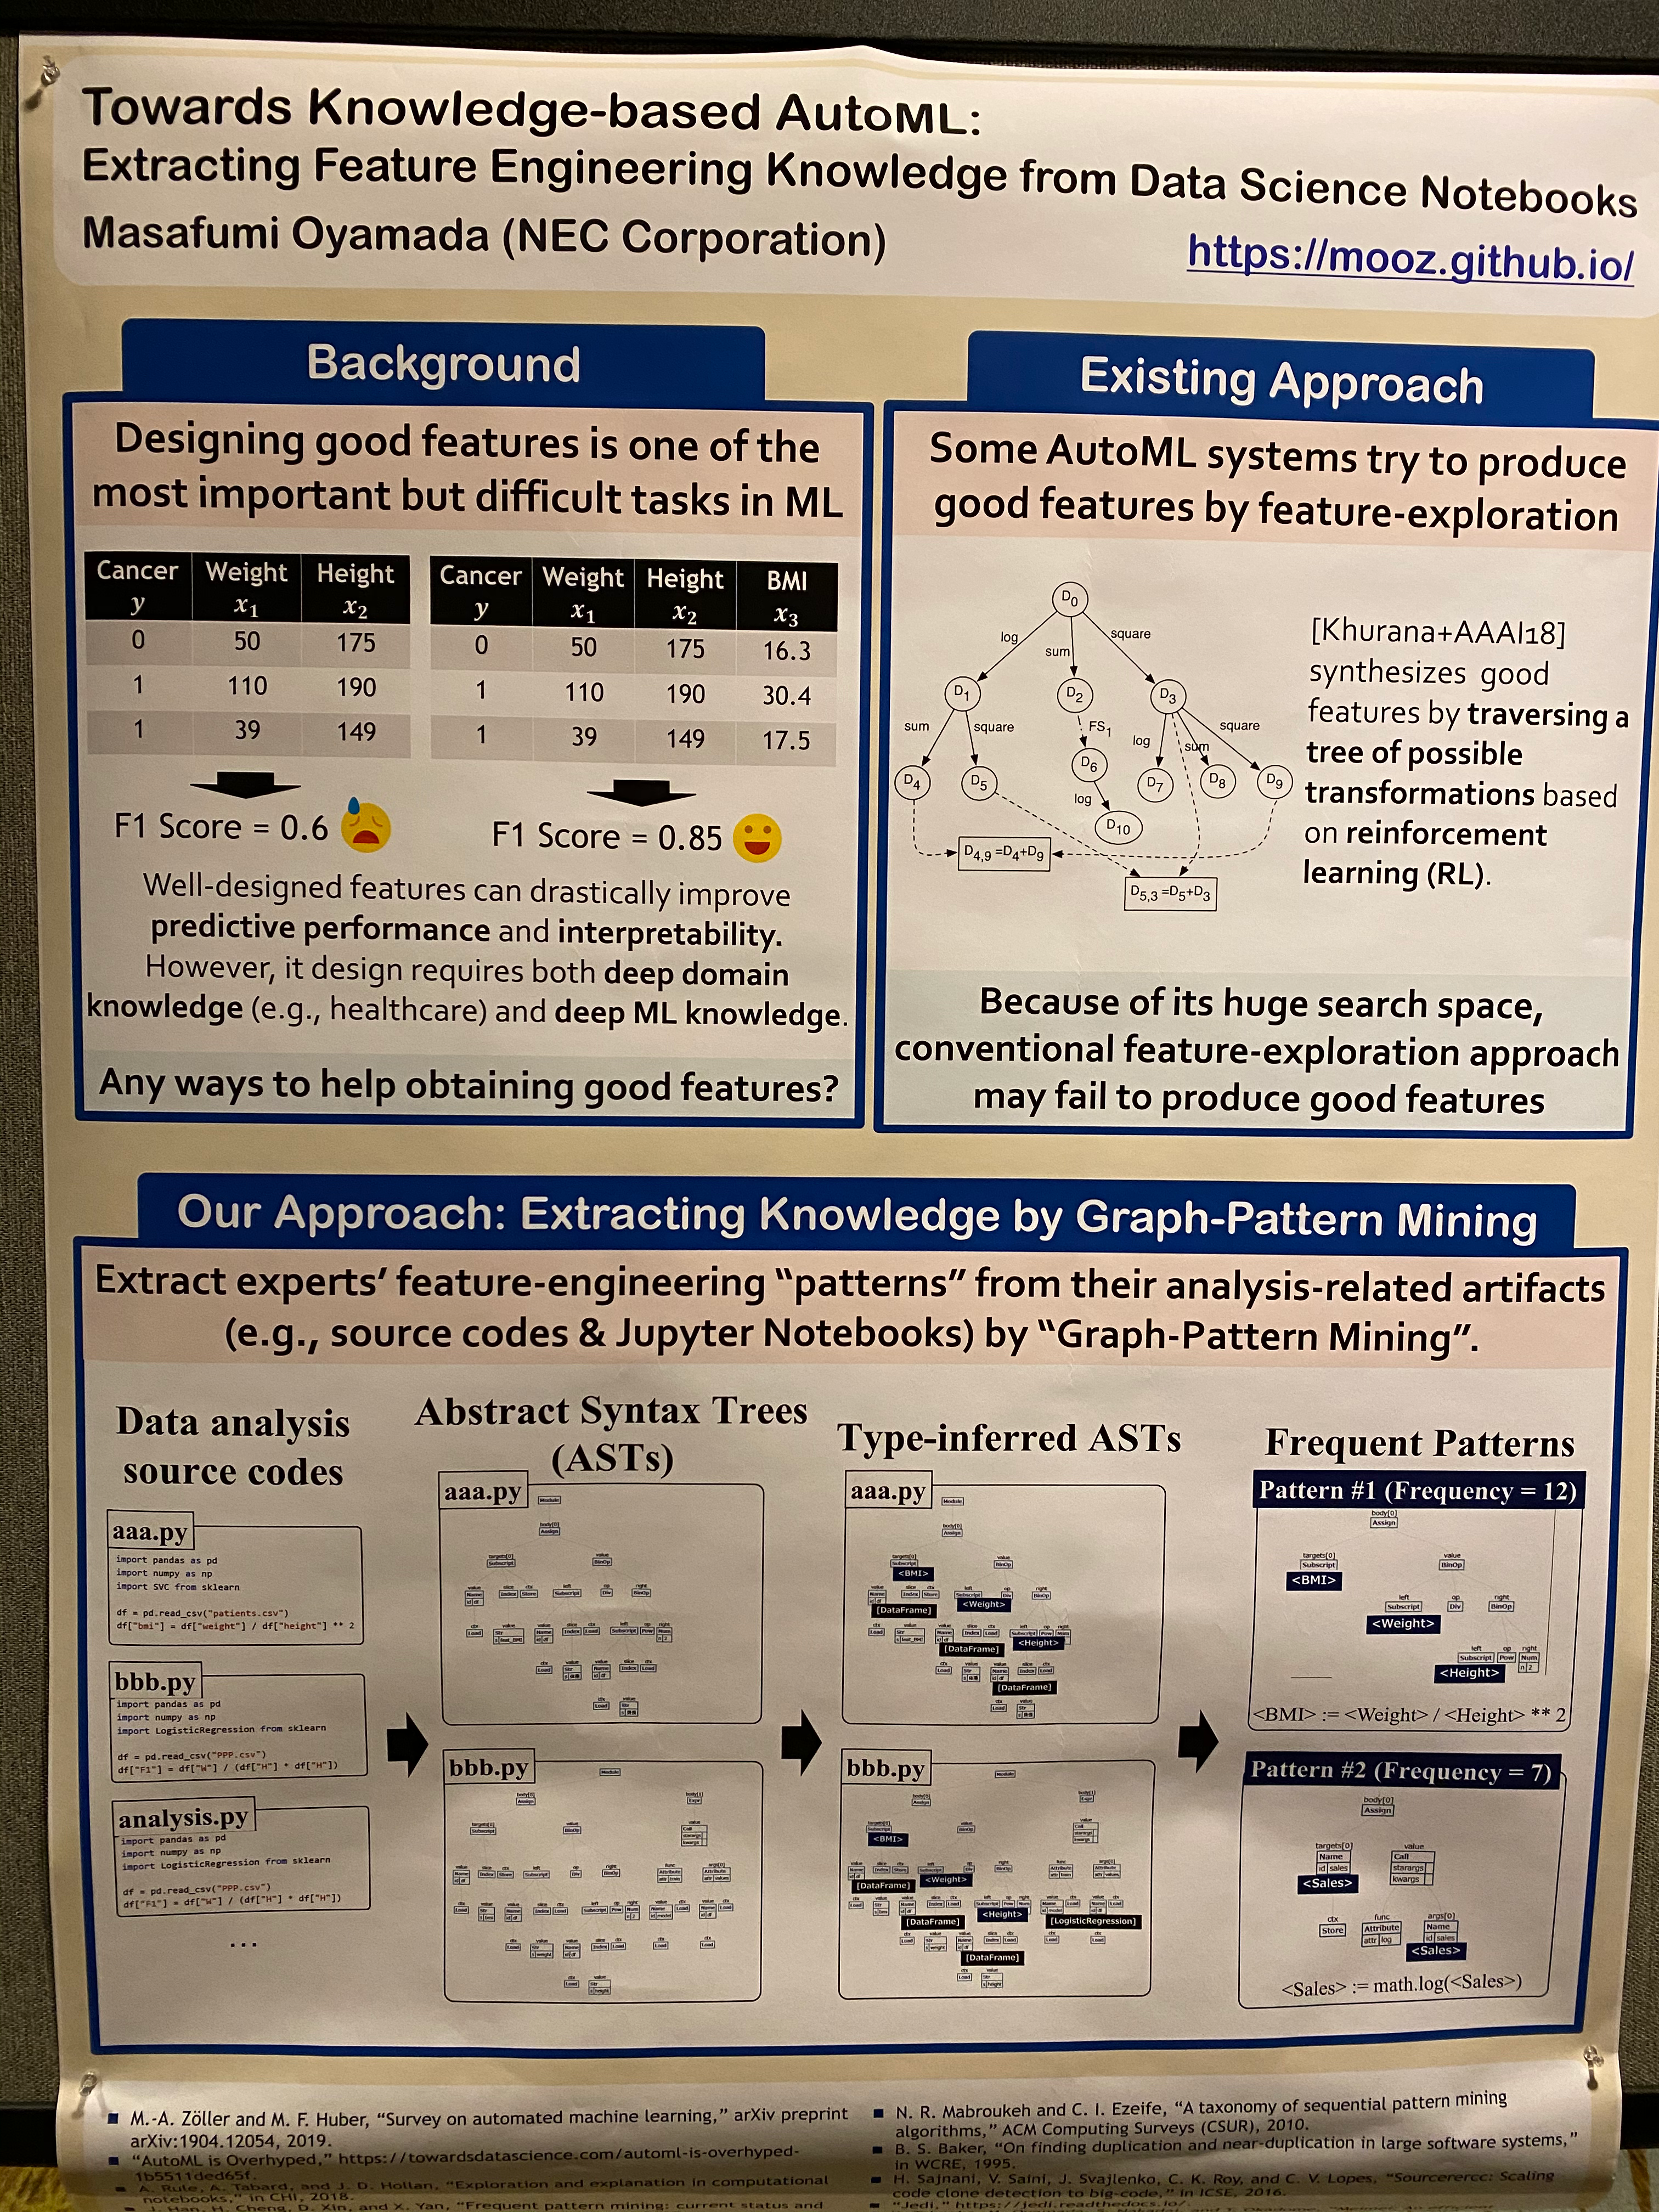
\includegraphics[width=120mm]{images/feature_engineering.png}
    \caption{Feature engineering with RL}
    \label{fig:my_label}
\end{figure}{}



\begin{figure}[!ht]
    \centering
    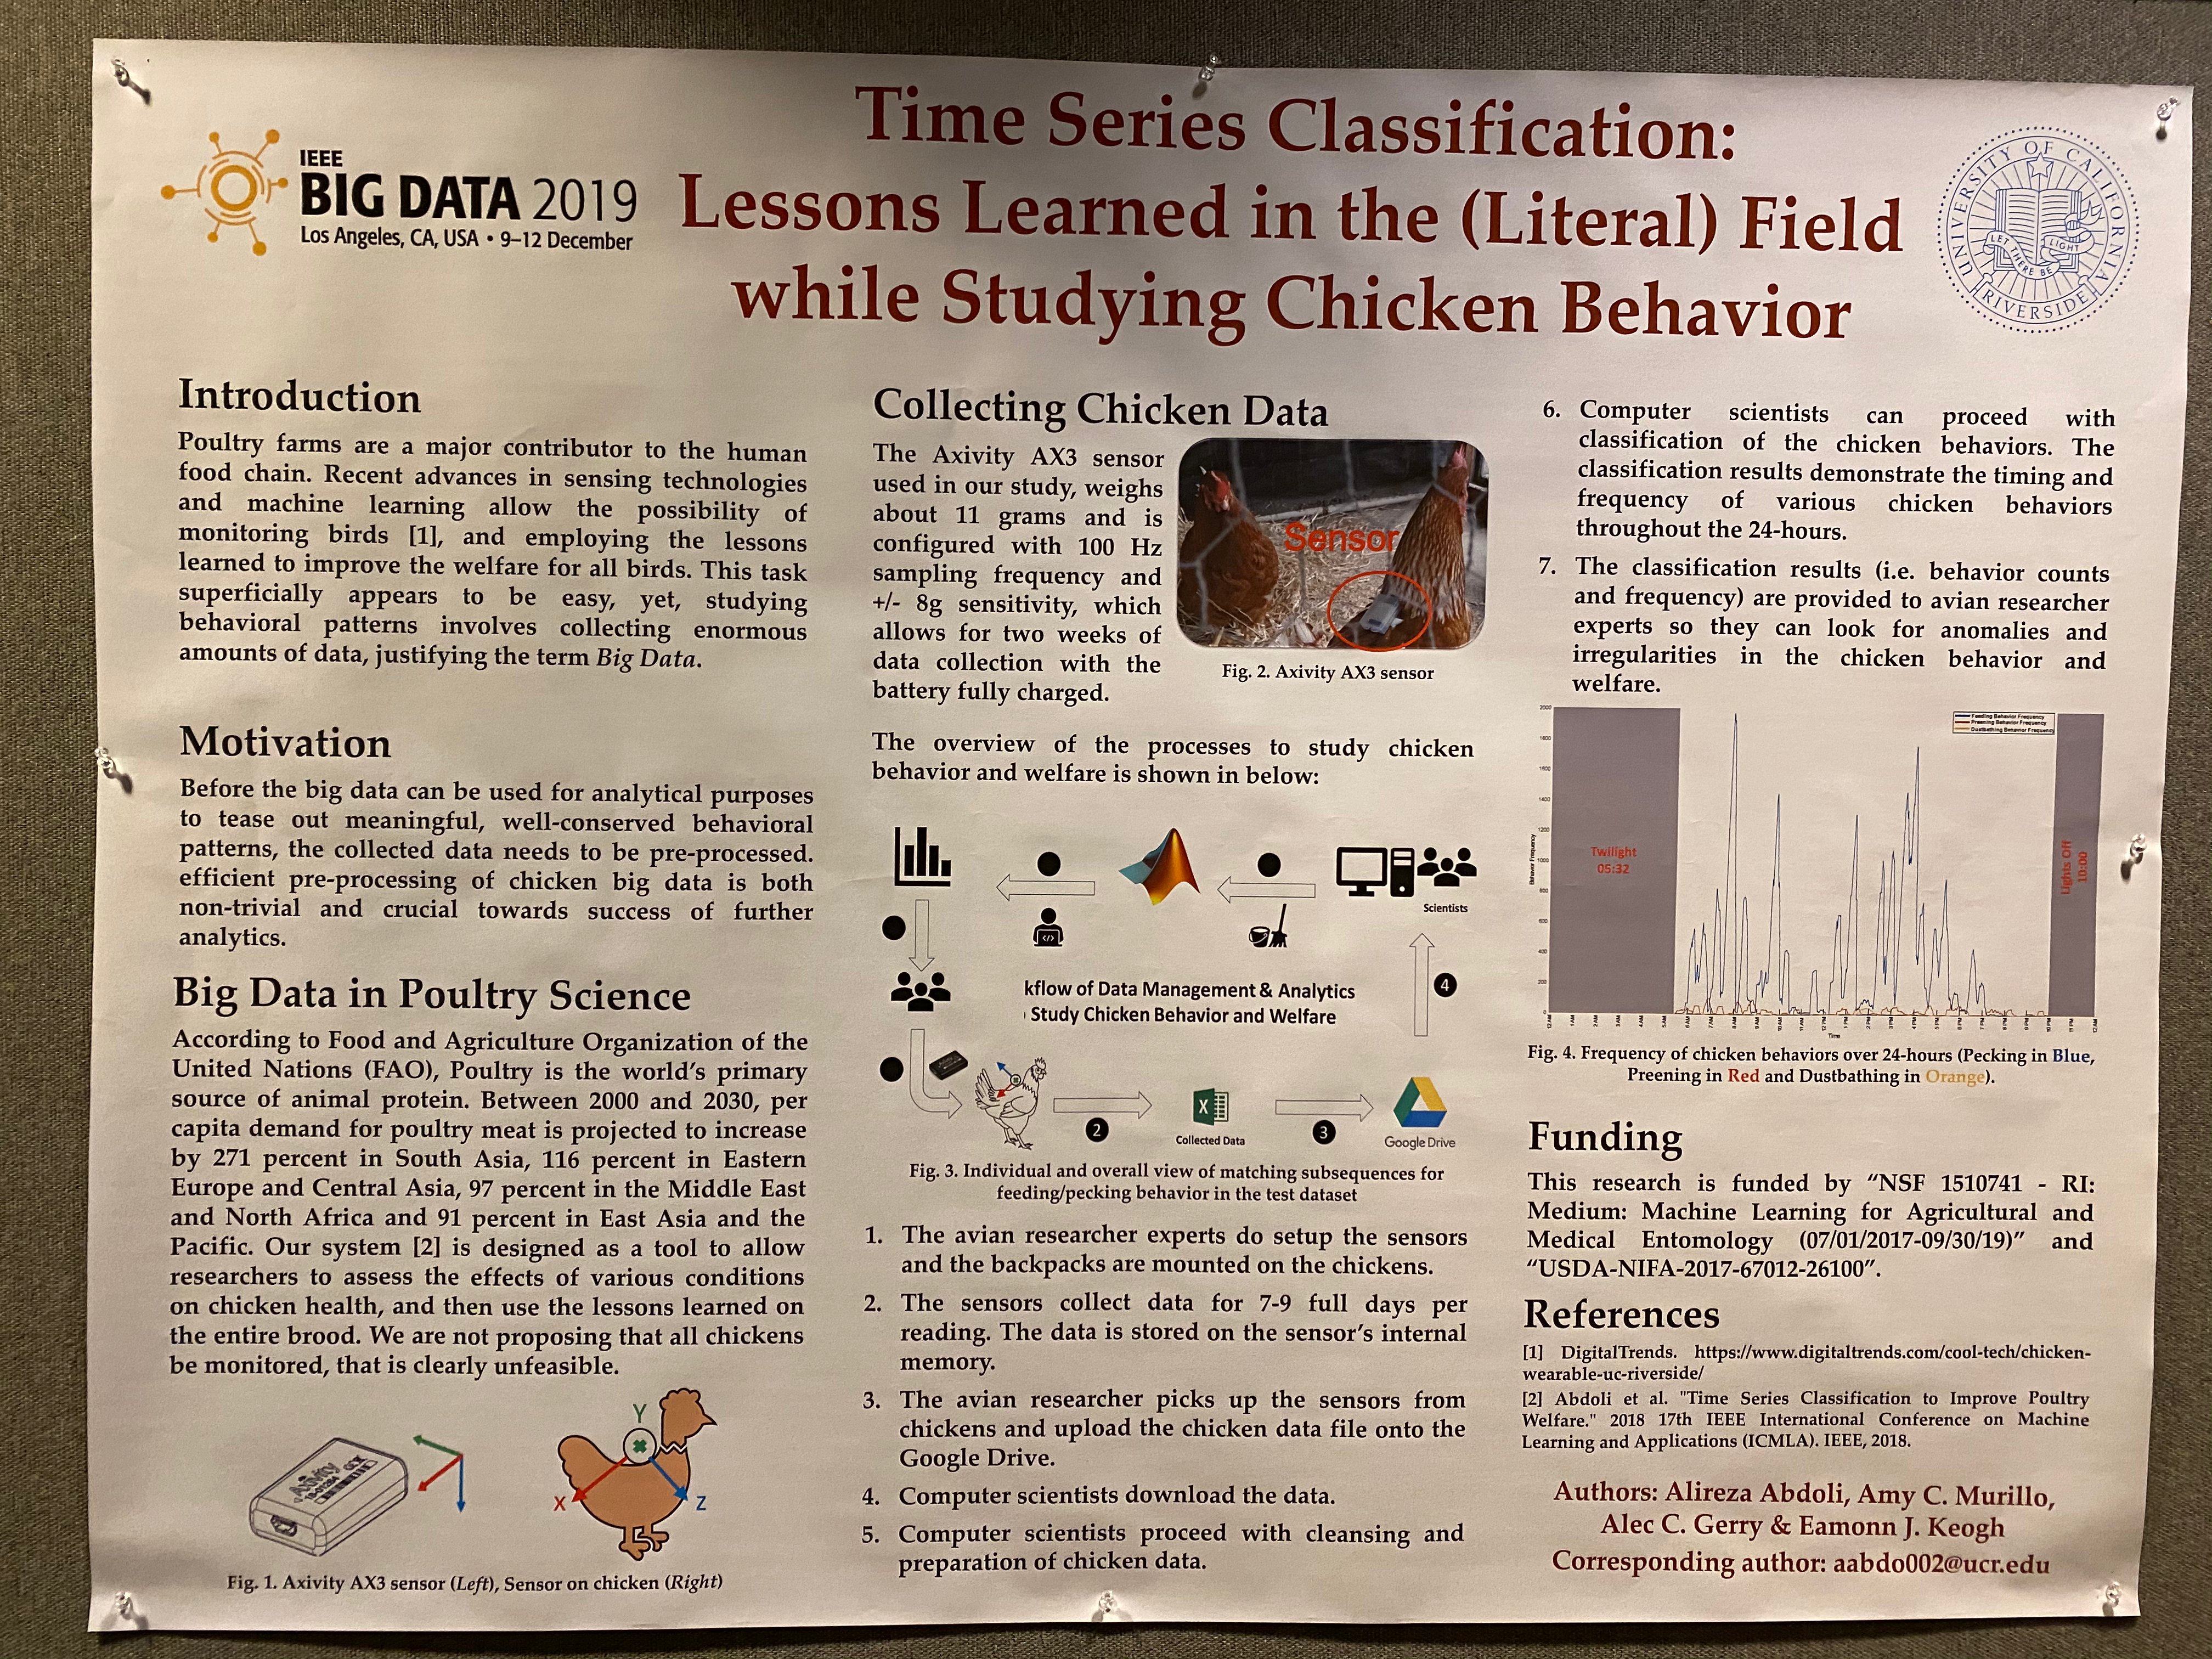
\includegraphics[width=120mm]{images/sarp_chicken.png}
    \caption{SARP on chicken?}
    \label{fig:my_label}
\end{figure}{}

\begin{figure}[!ht]
    \centering
    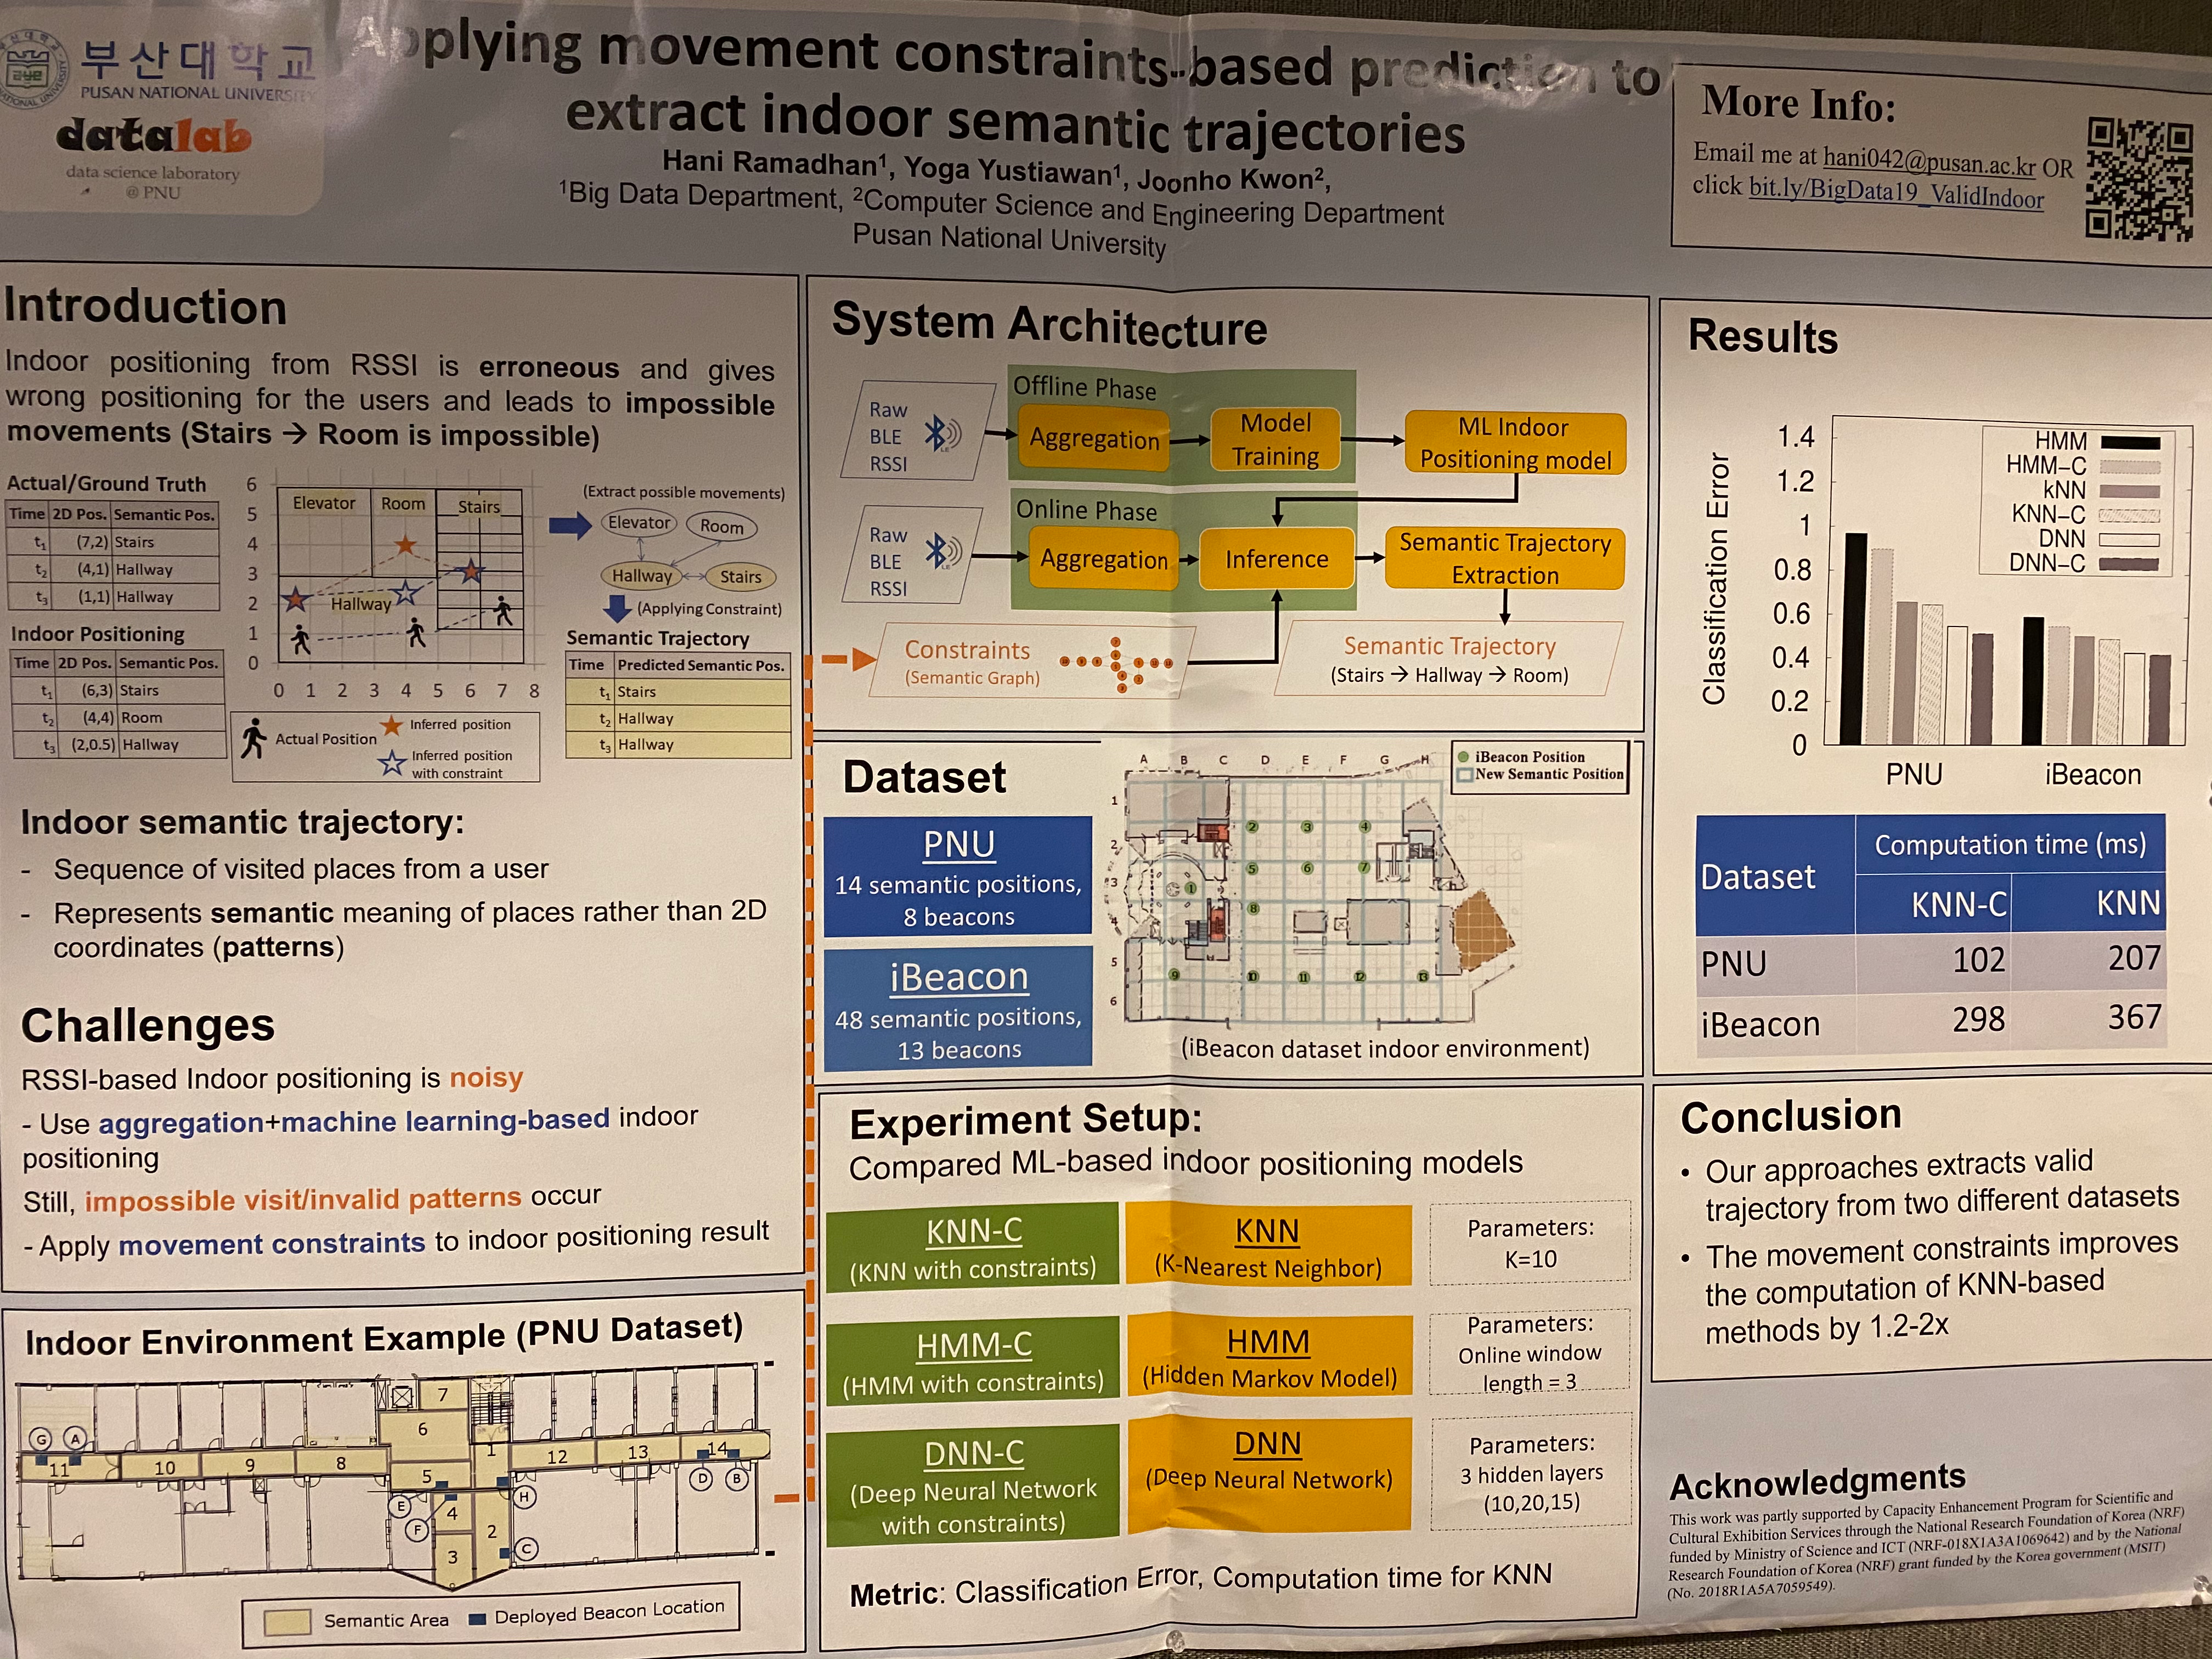
\includegraphics[width=120mm]{images/indoor.png}
    \caption{Indoor localization/trajectory prediction}
    \label{fig:my_label}
\end{figure}{}

\idea{Feature selection: using RL to do the feature selection, define a action graph where each feature is selected or not. then test the classifier on a small subset of the dataset. Then iterate the process.}

\idea{Causal discovery: similarly, can I use RL to find the causality. By deleting or adding the causal relations between the variables.}

\subsection{Complex Big Data Applications}

\idea{Multitask learning: can we apply MTL in FPG and Cardinal dataset?}

\subsection{New Computational Models for Big Data}

\subsubsection{Activation ensembles deep neural network}

$y_i=\sum_{i}\alpha_ih_i(\vec{x})$ where $h_i(\vec{x})$ is the activation function here (e.g., relu, tanh, etc.), and $\alpha$ is trainable. 

The optimization problem is defined as:

$$
minimize: \frac{1}{2}\sum(\hat{\alpha} - \alpha)^2
$$

$$
subject\ to: \sum_{n}\alpha_i = 1; \alpha_i \leq 0
$$

The results show that improvements are small but consistent in all experiments.

\subsubsection{Online federated learning}

For distributed data that are subject to privacy or security where data centralization is not possible.\\

$\ra$ Traditional approach: users' data from end device to central database\\
$\ra$ Proposed approach: models are built on end devices and the training parameters are transferred to central server. \\

\note{iPhone probably is deployed with this technology when learning ml models}

Federated multitask learning: each mobile device is considered as a separate task. \\

Federated multitask learning is formulated as an optimization problem:

\begin{figure}
    \centering
    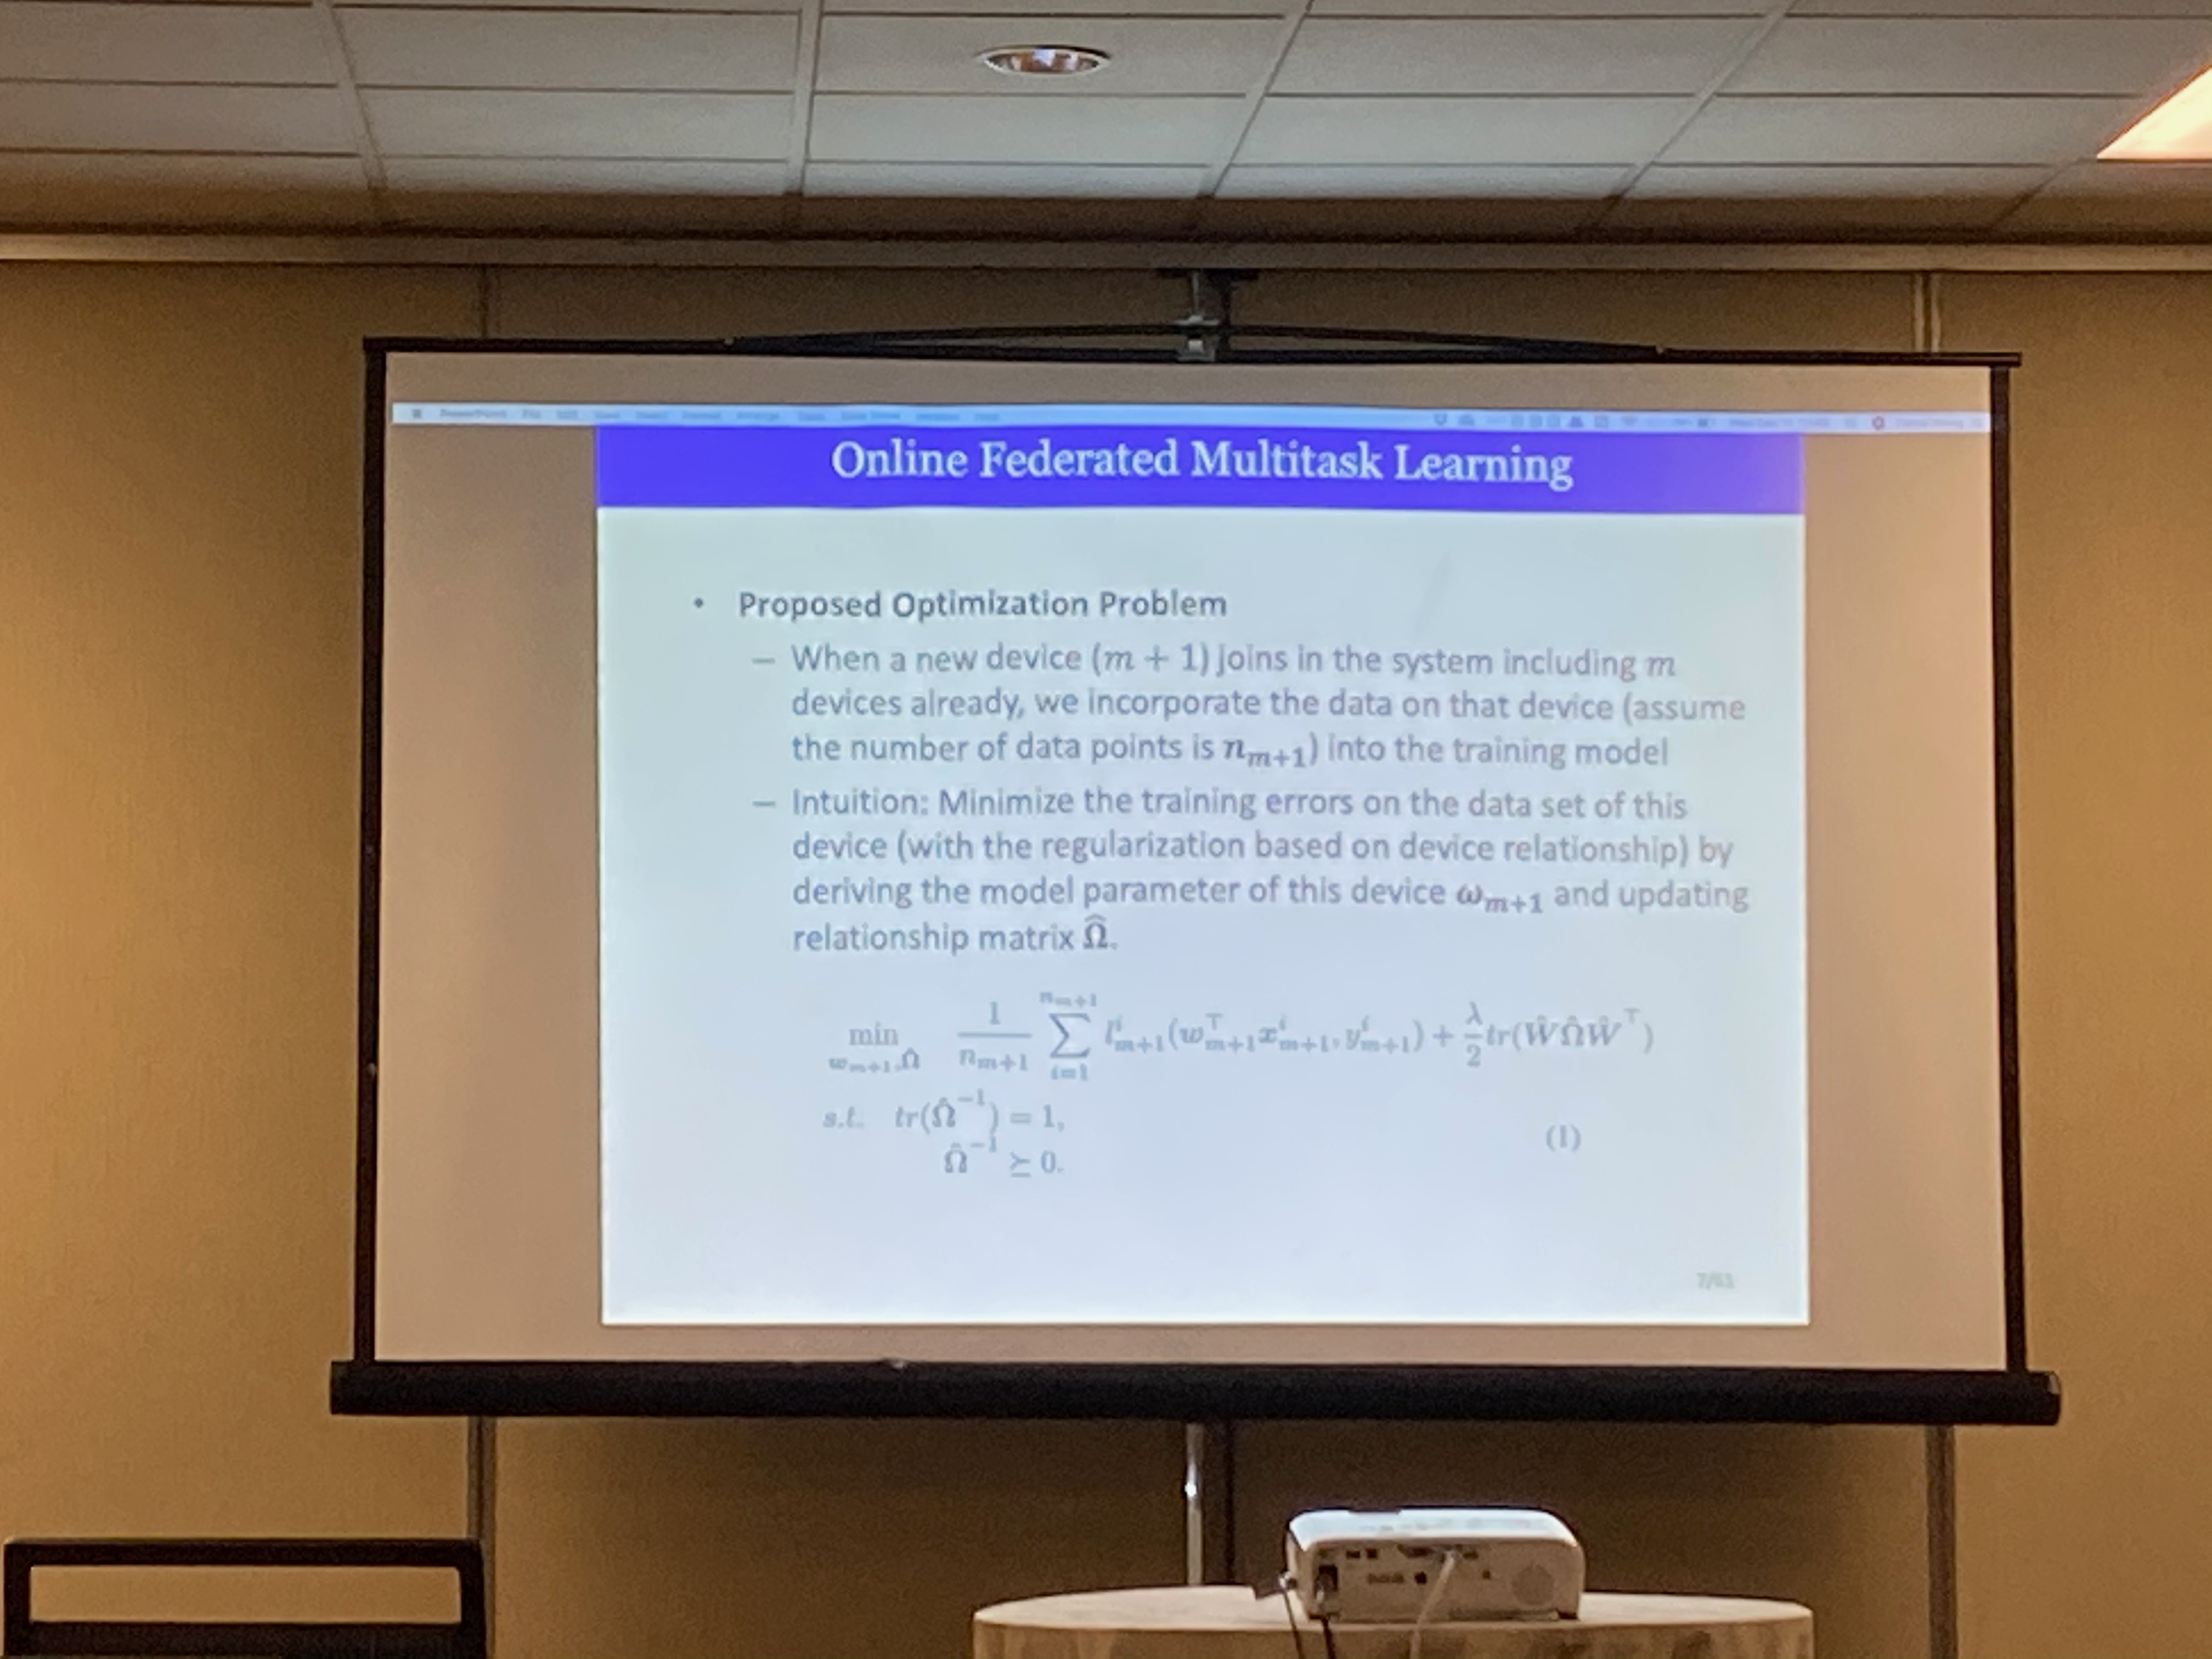
\includegraphics[width=120mm]{images/online_federated.png}
    \caption{Online federated as an optimization problem}
    \label{fig:my_label}
\end{figure}{}

{\bf Datasets}:

\begin{itemize}
    \item Human Activity Recognition 
    \item Eating Habit Monitoring
\end{itemize}{}



\subsection{Taming the complex unstructured data mining}

The speaker is Jiawei Han\footnote{\url{https://www.leiphone.com/news/201807/CWmEgpJaQmbHjkex.html}}.\\

$\ra$ Entity and relation extraction from text corpus. 

\idea{Can I  use entities and  relation extractions to mine causality relations in non-numeric dataset, such as text or images}

\spacerule

\subsection{Keynote: Data Commons}

\label{section:datacommmons}

The speaker is Guha from Google.\\

We have math equations models for areas that are simple but not for the domains that are complex.\\

Data Commons is a service where Google keeps a variety of datasets and provide open public access to them for data analytic. It's built with Python APIs. See \url{https://colab.research.google.com/drive/1qCPZZD0MPWx6CC34wFVJc_9B2-q0F-h_}\\

\remark{Basically, Data Commons is a better version of UCI machine learning repo.}

\note{Data journalism seems to be an interesting job}

\remark{\url{Schema.org} is a tool/service for extracting structured data from website and this might be very helpful in mining web/email information and creating datasets.}

\spacerule

\subsection{Panel: Addressing Big Data Heterogeneity: Recent Advances and Challenges}

\subsubsection{Big Data in the IoT Context}

{\bf TIPPERS Testbed: Testbed for IoT-based Privacy-Preserving PERvasive Spaces}

\subsubsection{Addressing Big Data Heterogeneity Challenges: Transforming Massive Unstructured Big Data into Structured Knowledge}

over 80\% data is unstructured data (e.g., text, media)

{\bf how to automatically generate structures from text data?}


\spacerule

% ------------
% -- Thursday --
% ------------
\newpage
\section{Thursday Dec 12th, 2019: Main Conference}
This is the last day! Most of the regular/short paper presentation happen today.

\subsection{Short paper: Link and Graph Mining}

\subsubsection{LATTE: Application Oriented Social Network Embedding}
\ddef{Network embedding}{Map nodes in a network into a low-dimensional space}

\begin{figure}[ht!]
    \centering
    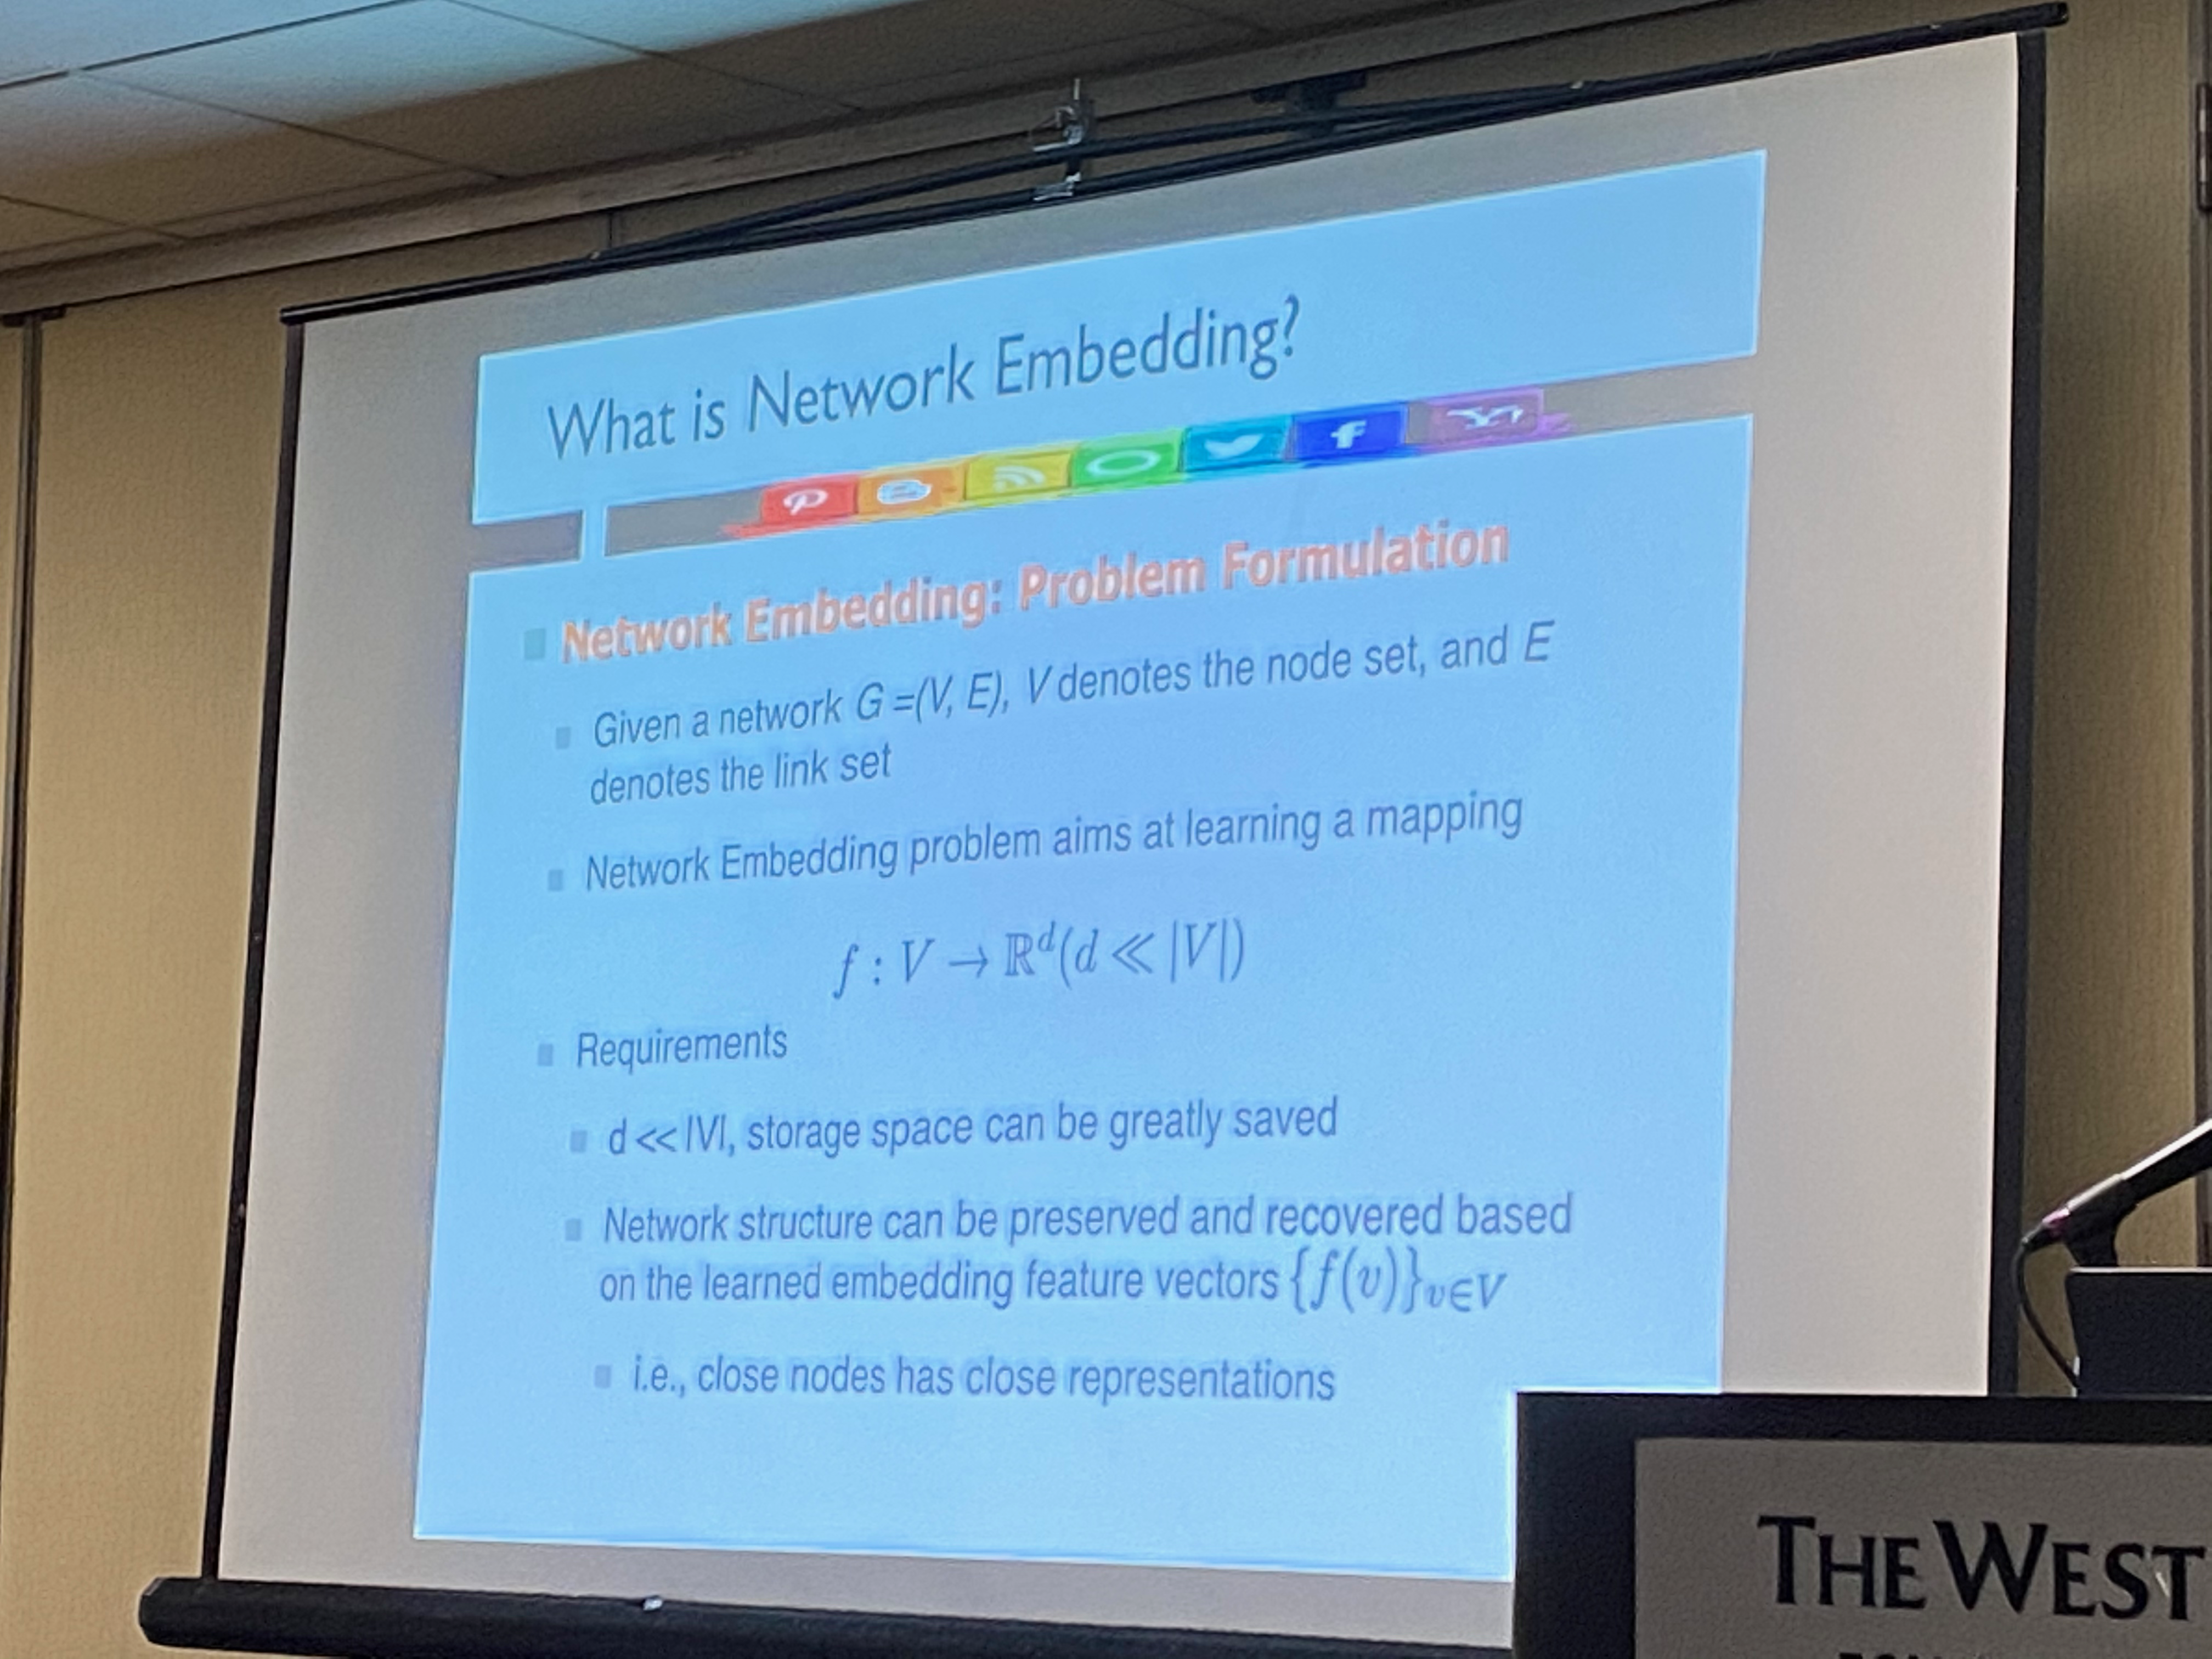
\includegraphics[width=120mm]{images/network_embedding.png}
    \caption{Network embedding}
    \label{fig:my_label}
\end{figure}{}


\subsubsection{BIGMat: A distributed affinity-perserving random walk strategy for instance mathcing on knowledge graph}

$\ra$ essentially a link prediction in knowledge graph by doing instance matching. Two nodes are matching candidate if they share at least one word, but this seems to be a big drawback.

\subsubsection{RecANt: Network-based Recruitment for Active Fake news Correction}

\begin{figure}[ht!]
    \centering
    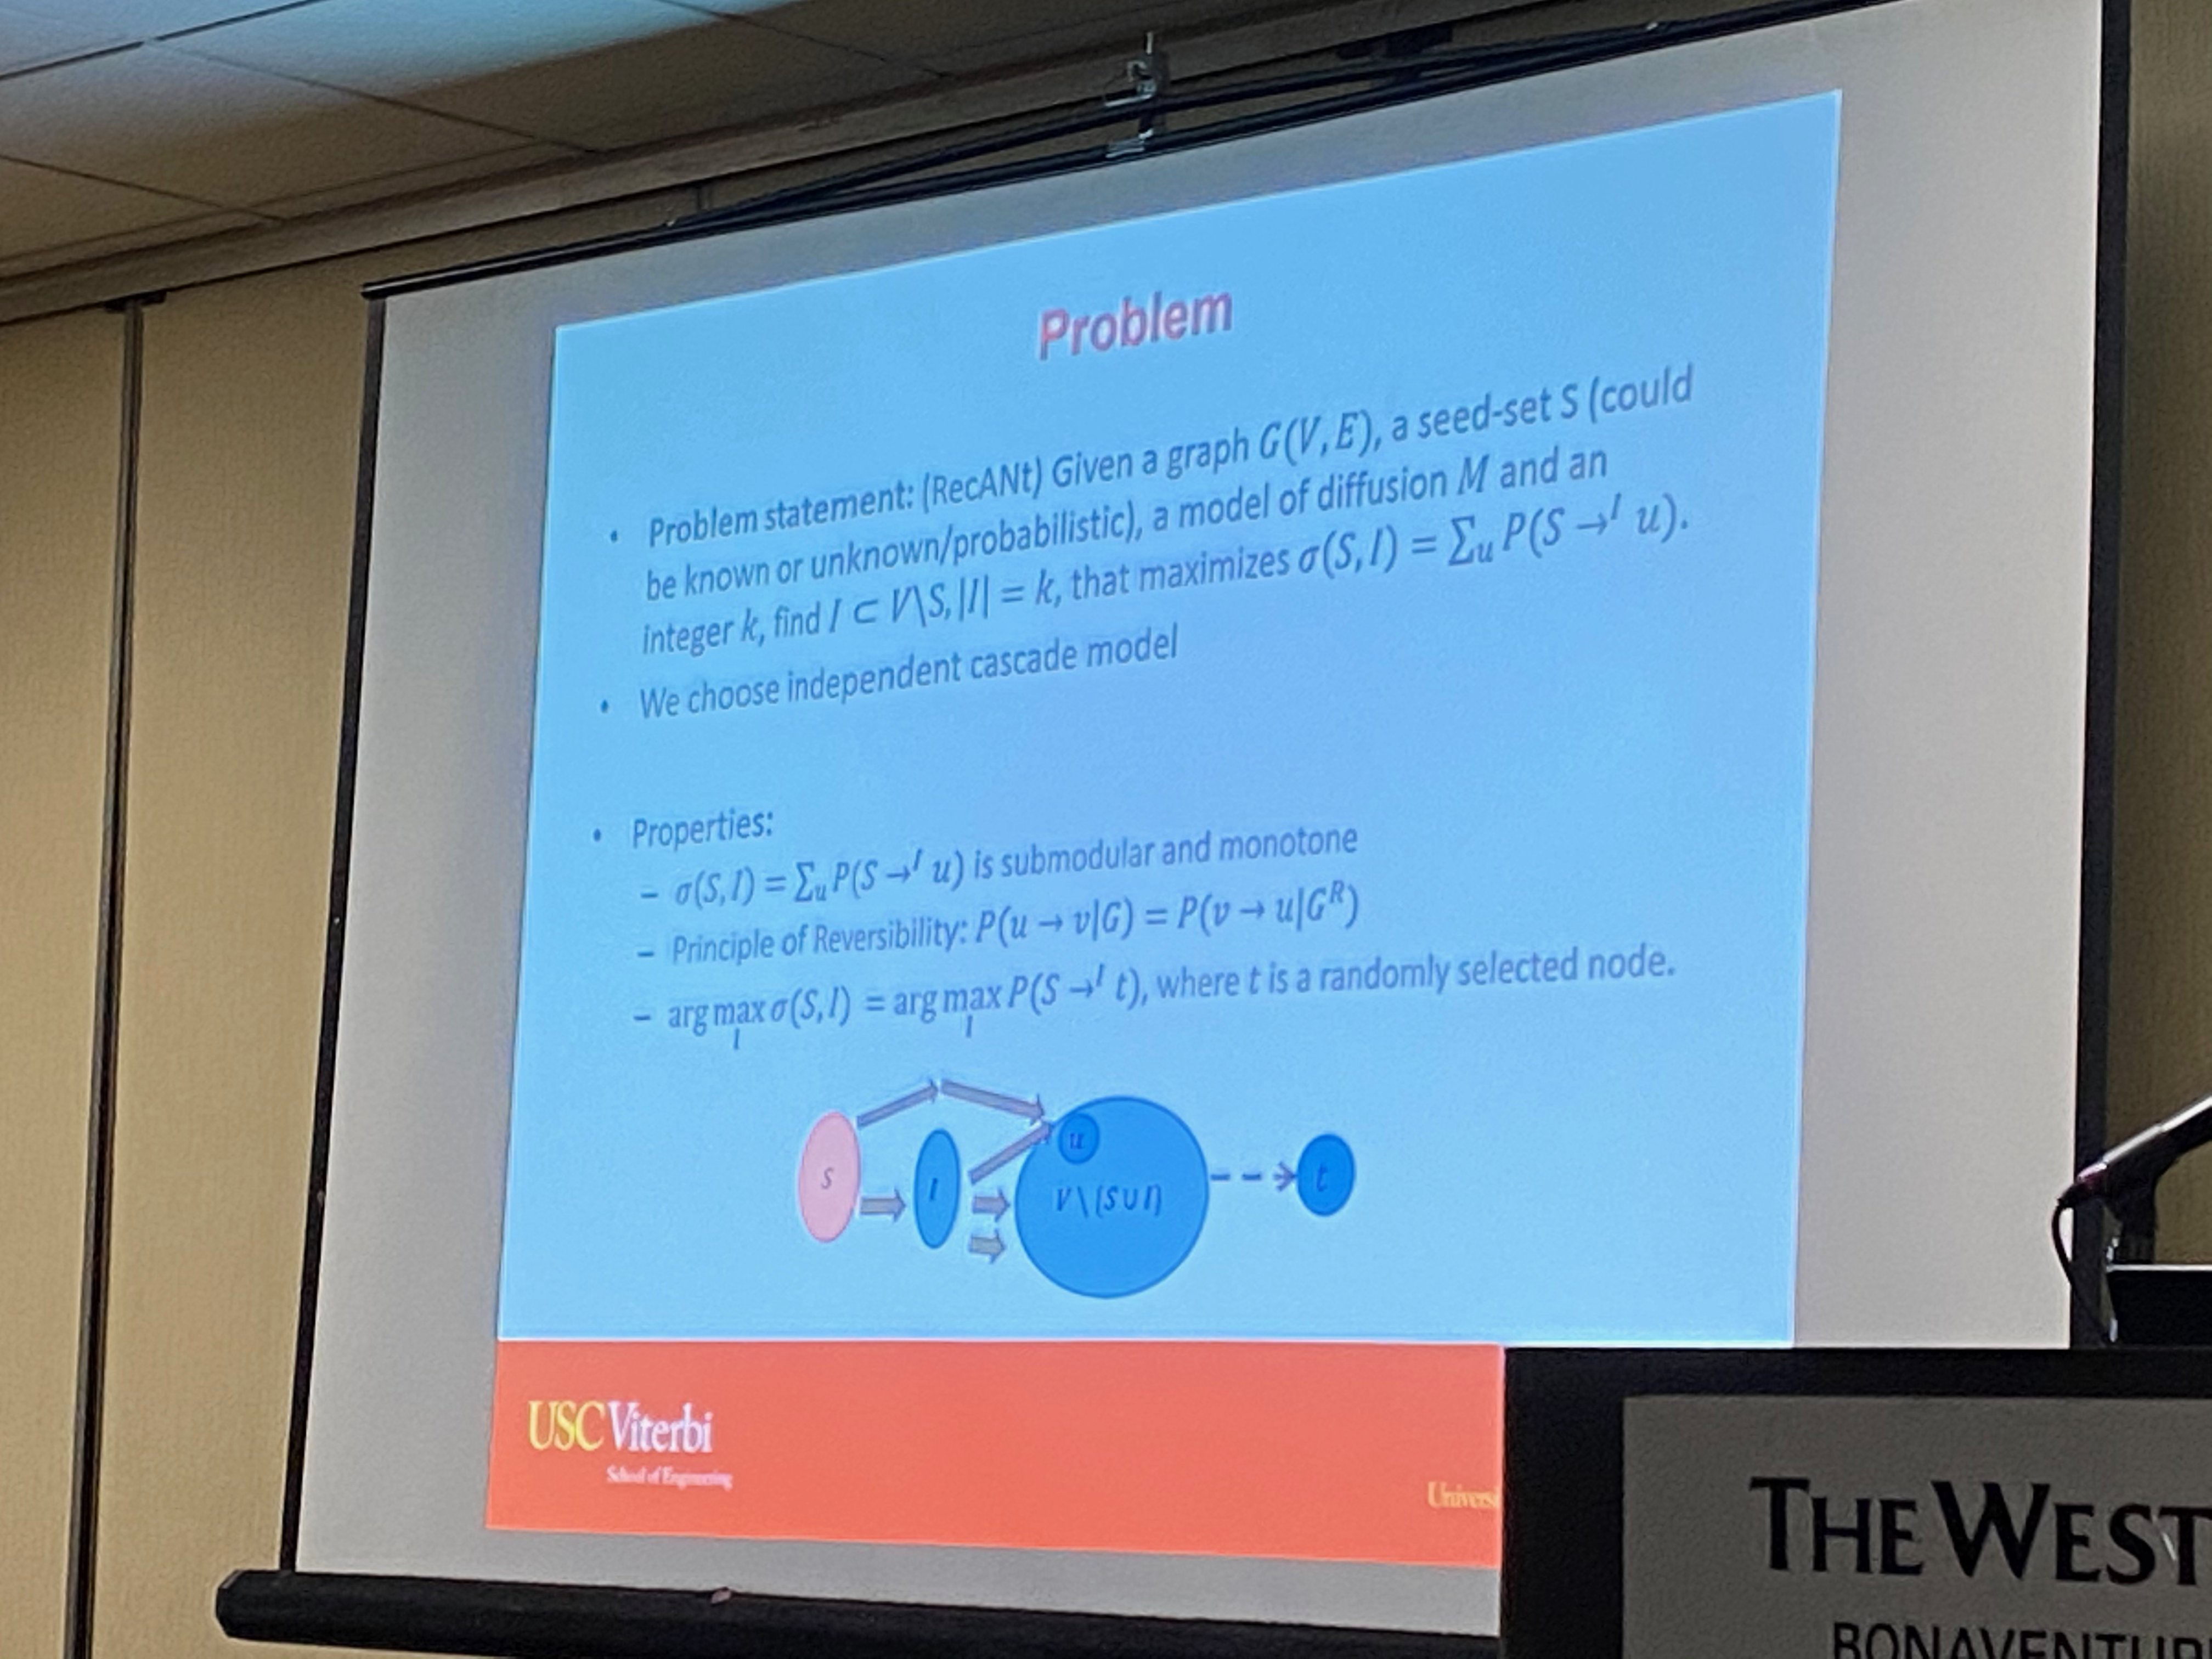
\includegraphics[width=120mm]{images/fake_news_prob.png}
    \caption{Network embedding}
    \label{fig:my_label}
\end{figure}{}

\begin{figure}[ht!]
    \centering
    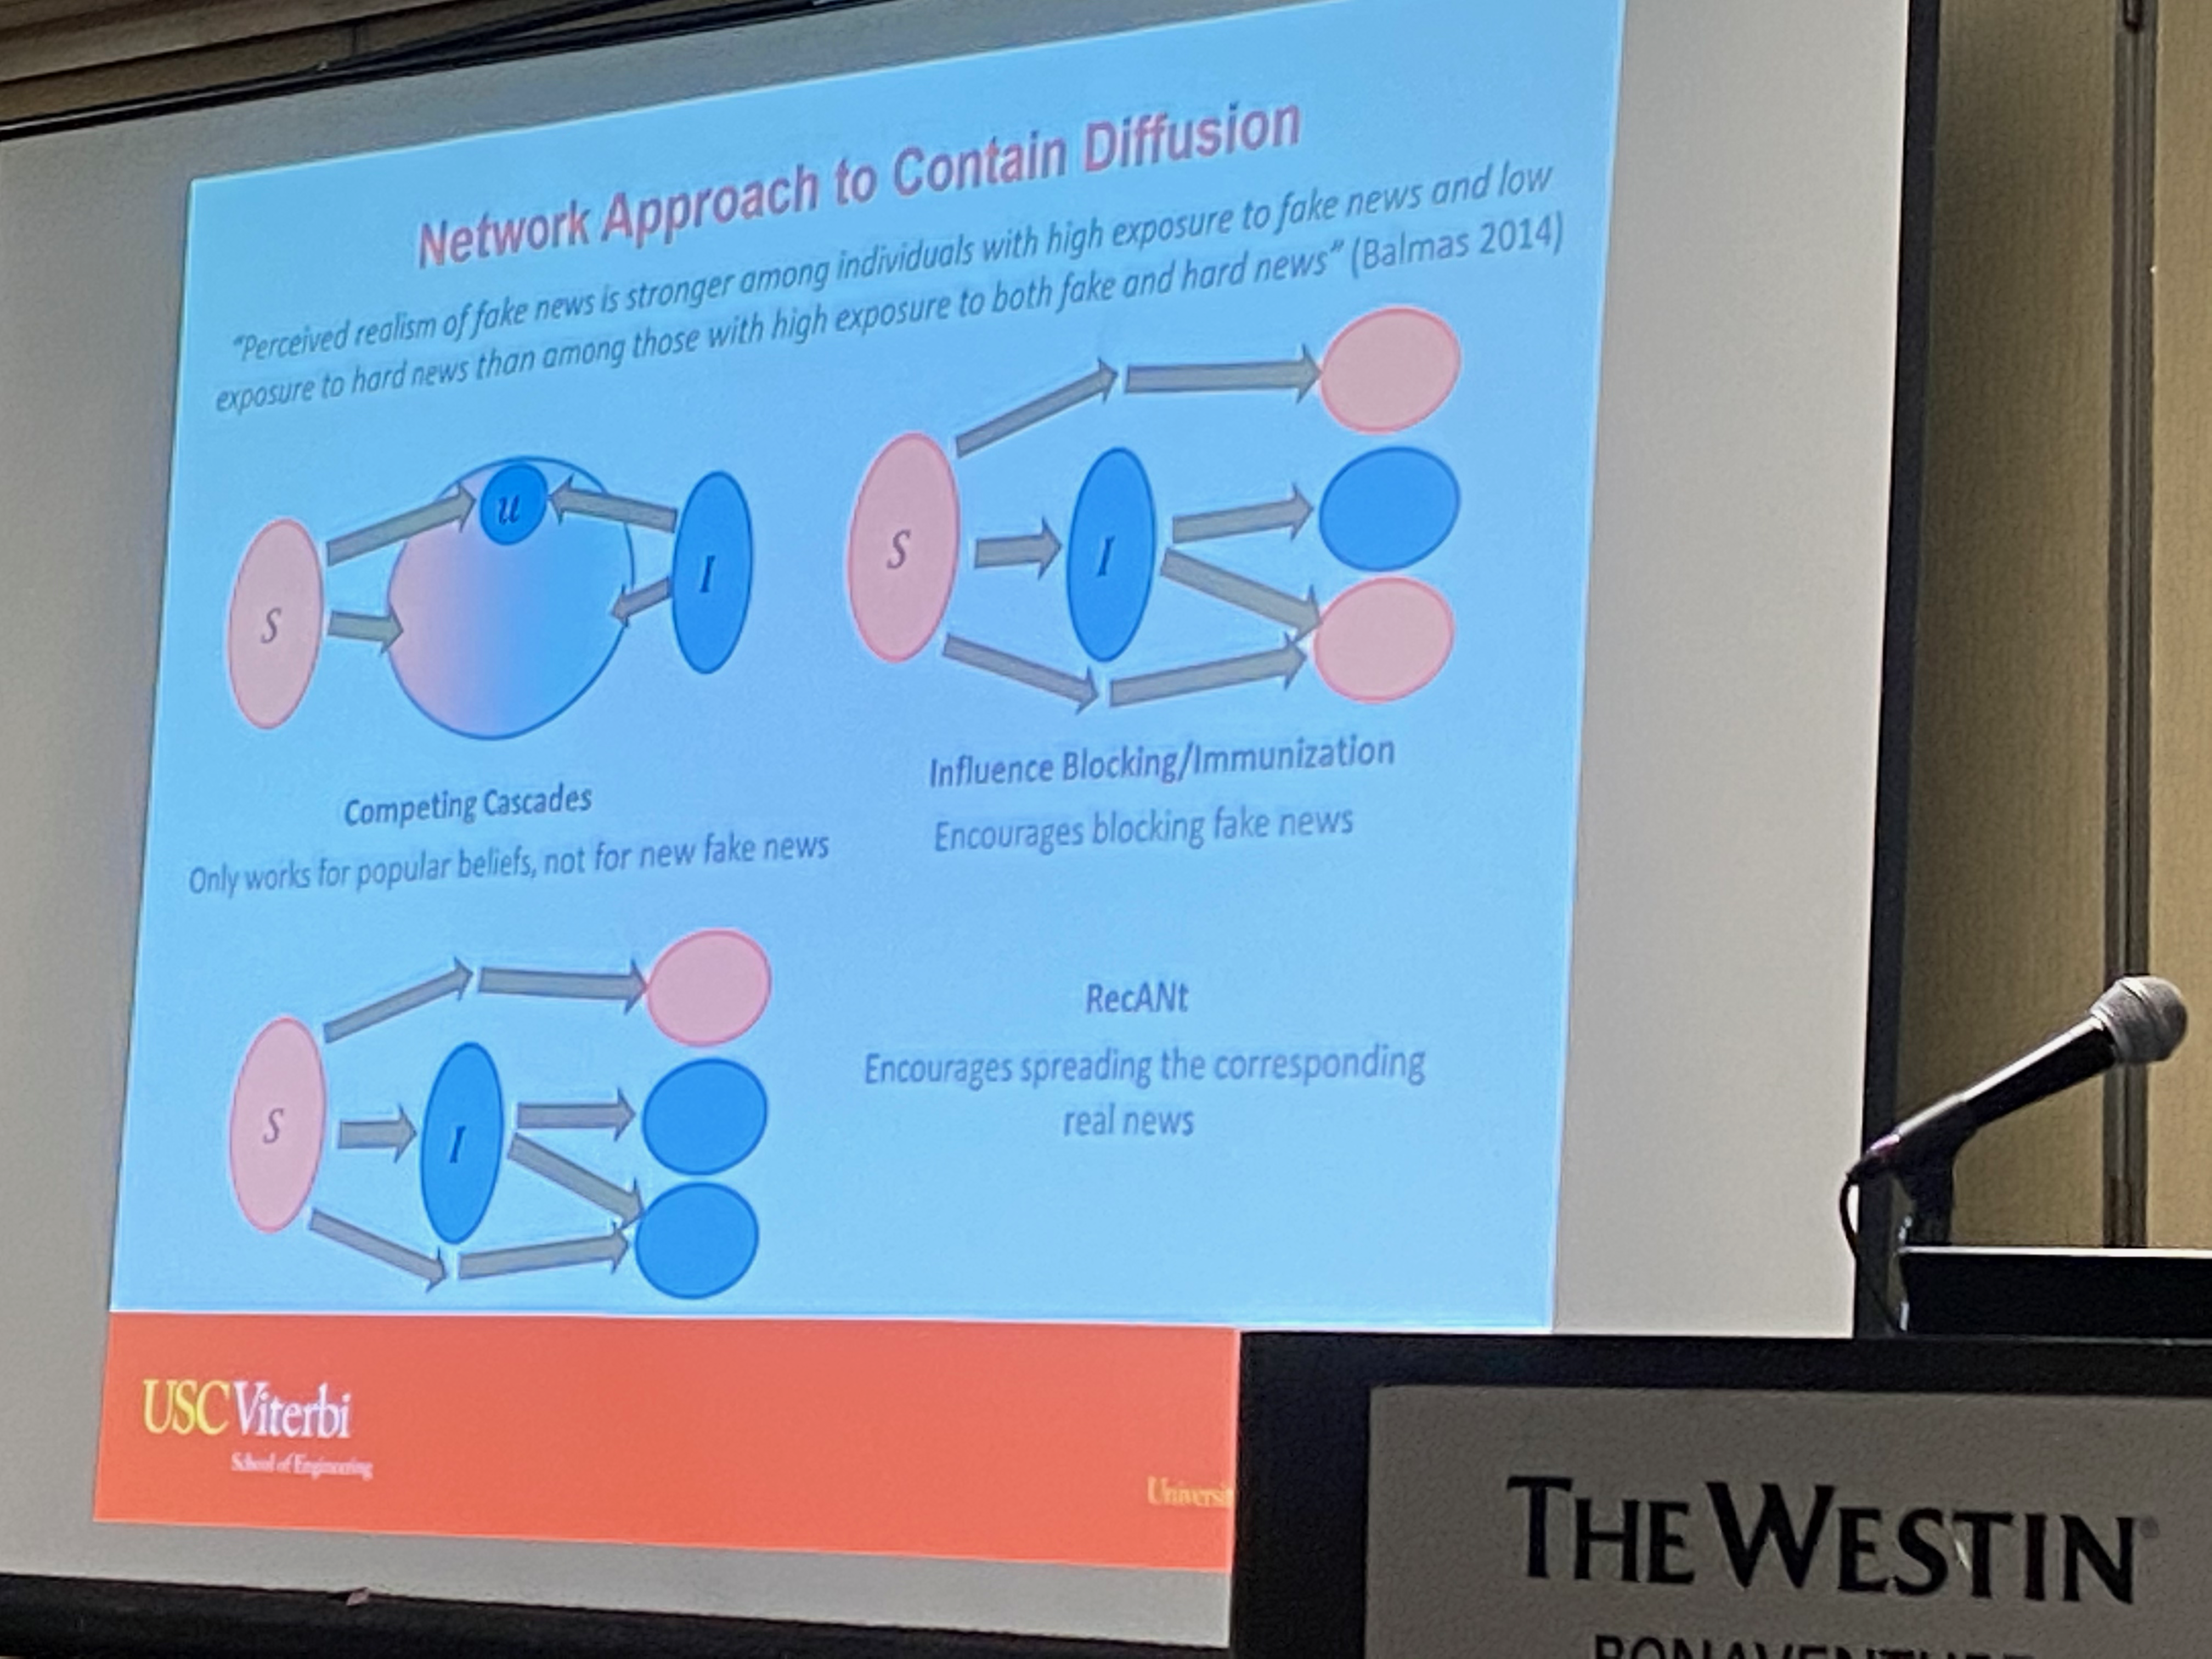
\includegraphics[width=120mm]{images/fake_news_diffusion.png}
    \caption{Network embedding}
    \label{fig:my_label}
\end{figure}{}

\subsubsection{Modelling Online Comment Threads from their Start}

{\bf Comment threads: take the form of a tree. The root is the original post. Comments are descendants of root}

\remark{Why we are trying to predict the comment threads?}

\begin{figure}
    \centering
    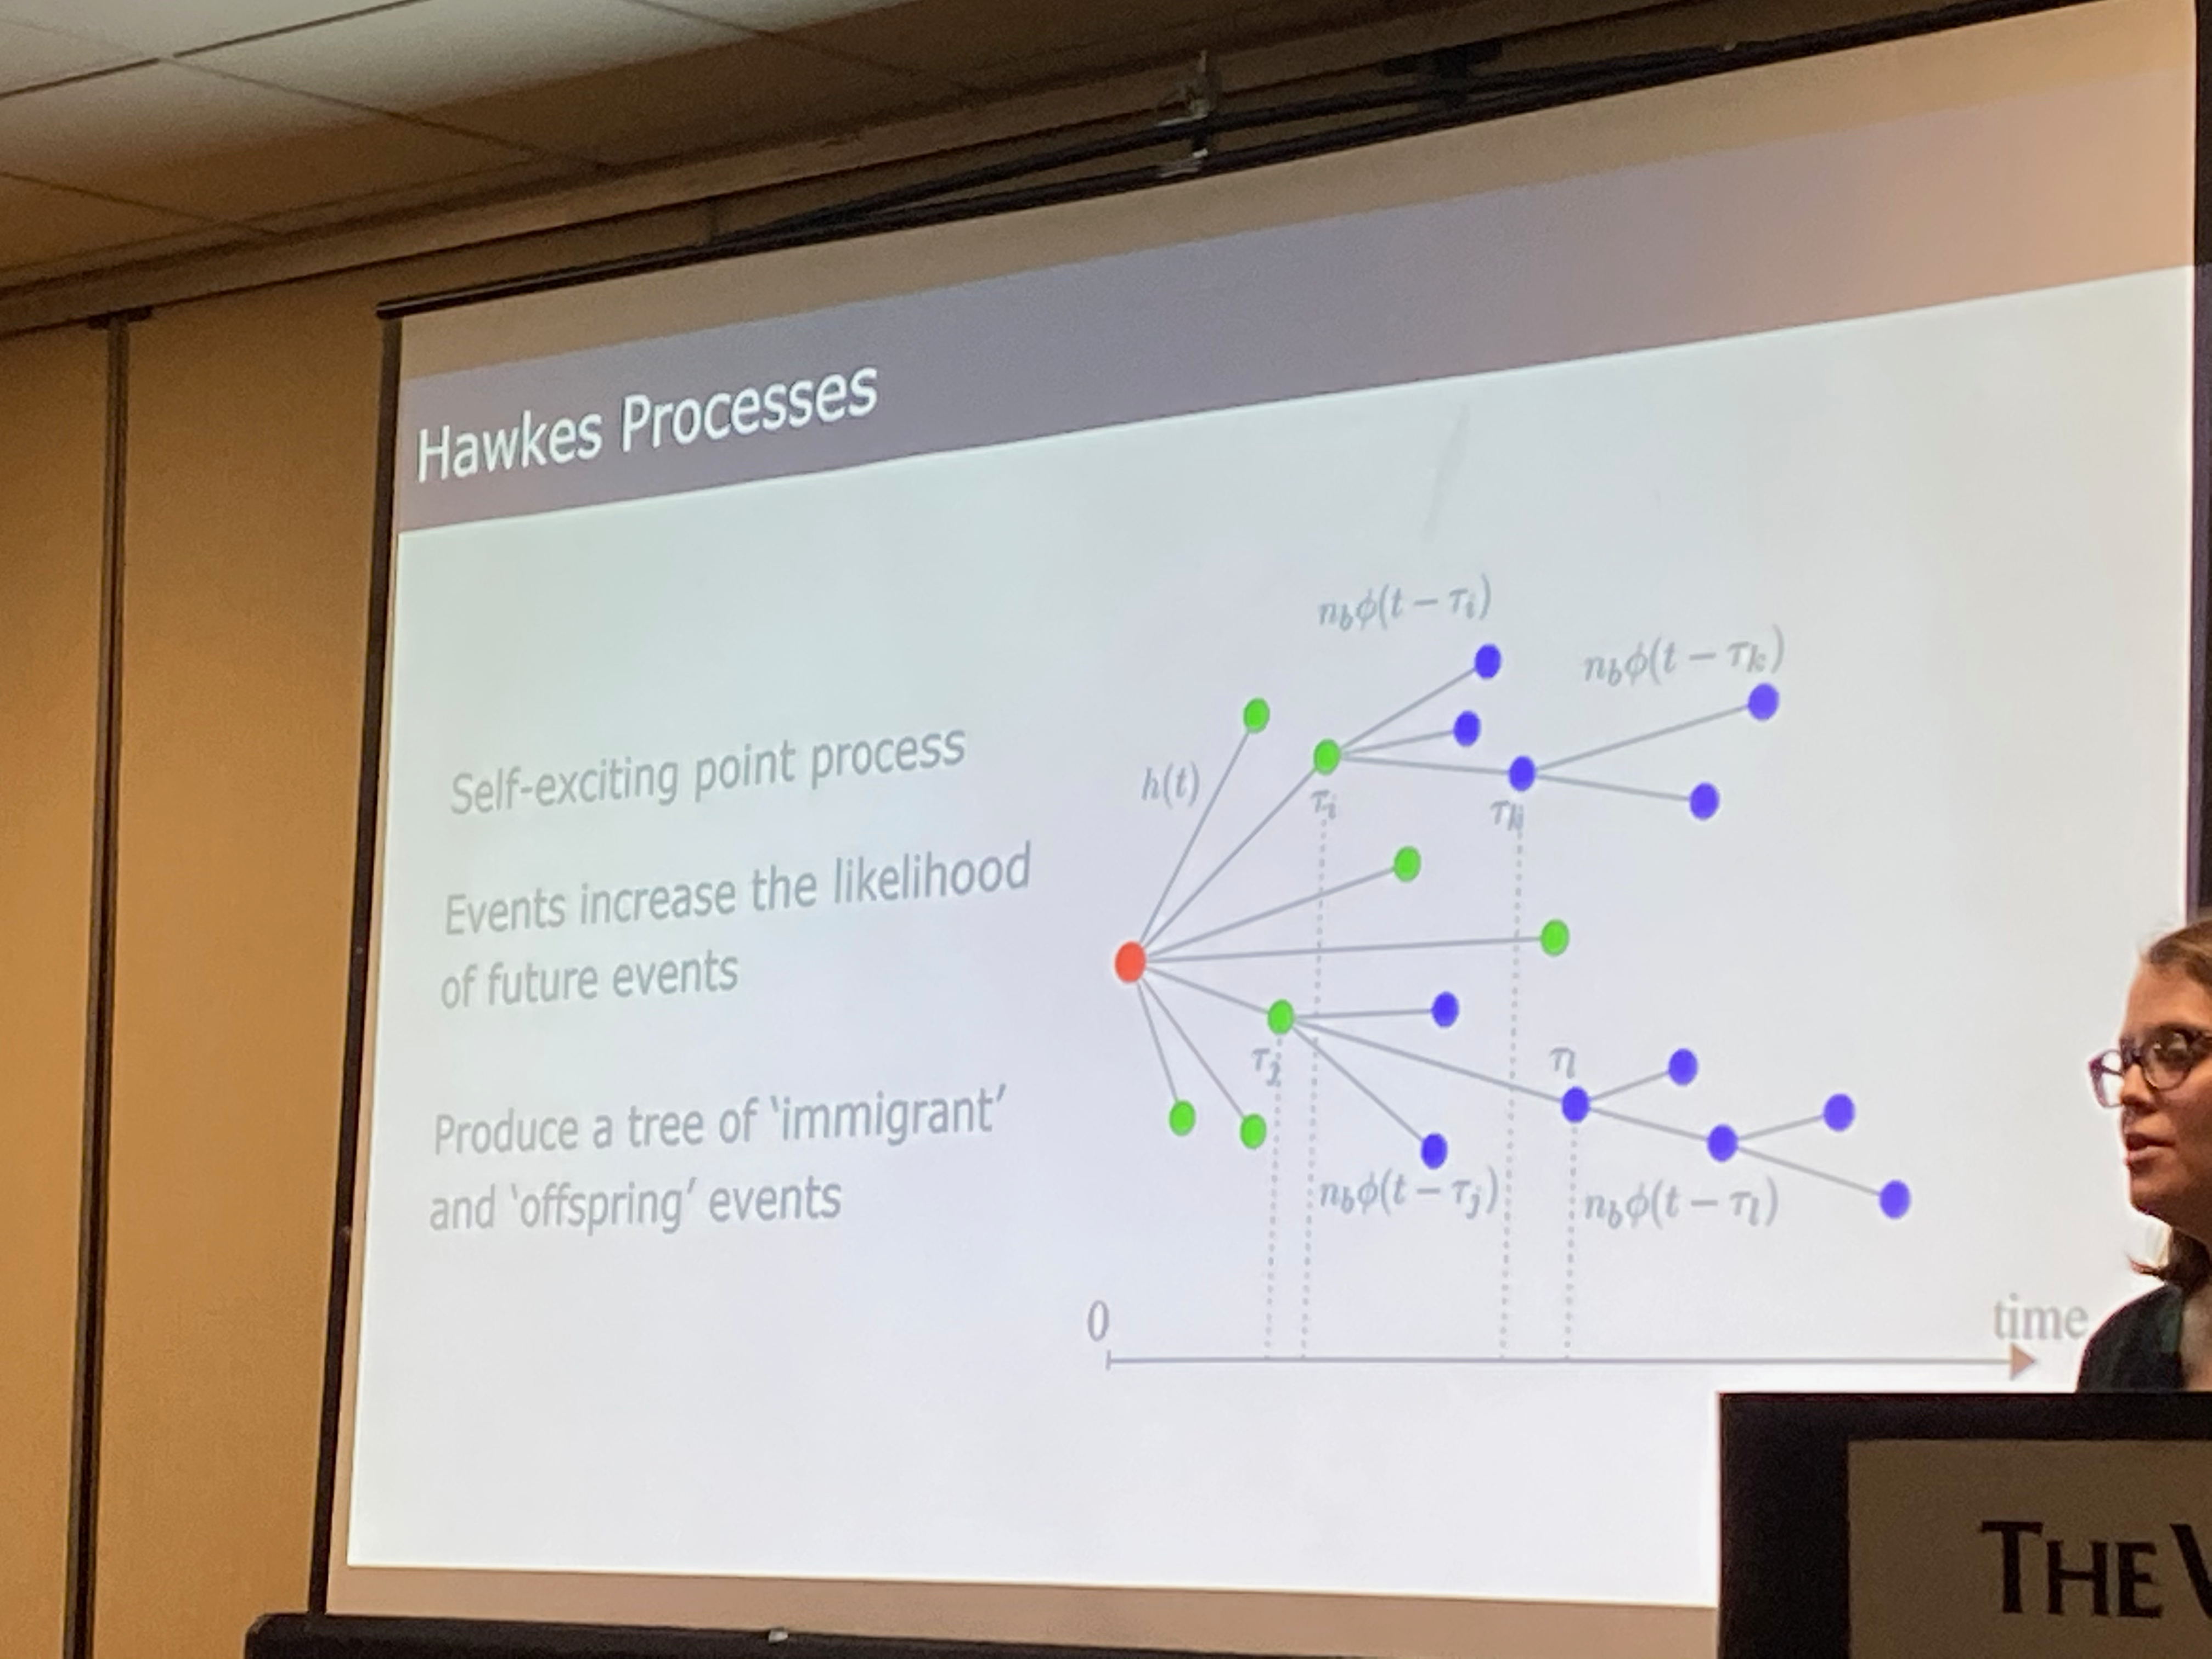
\includegraphics[width=120mm]{images/hawks.png}
    \caption{Hawks process}
    \label{fig:my_label}
\end{figure}{}

\begin{figure}
    \centering
    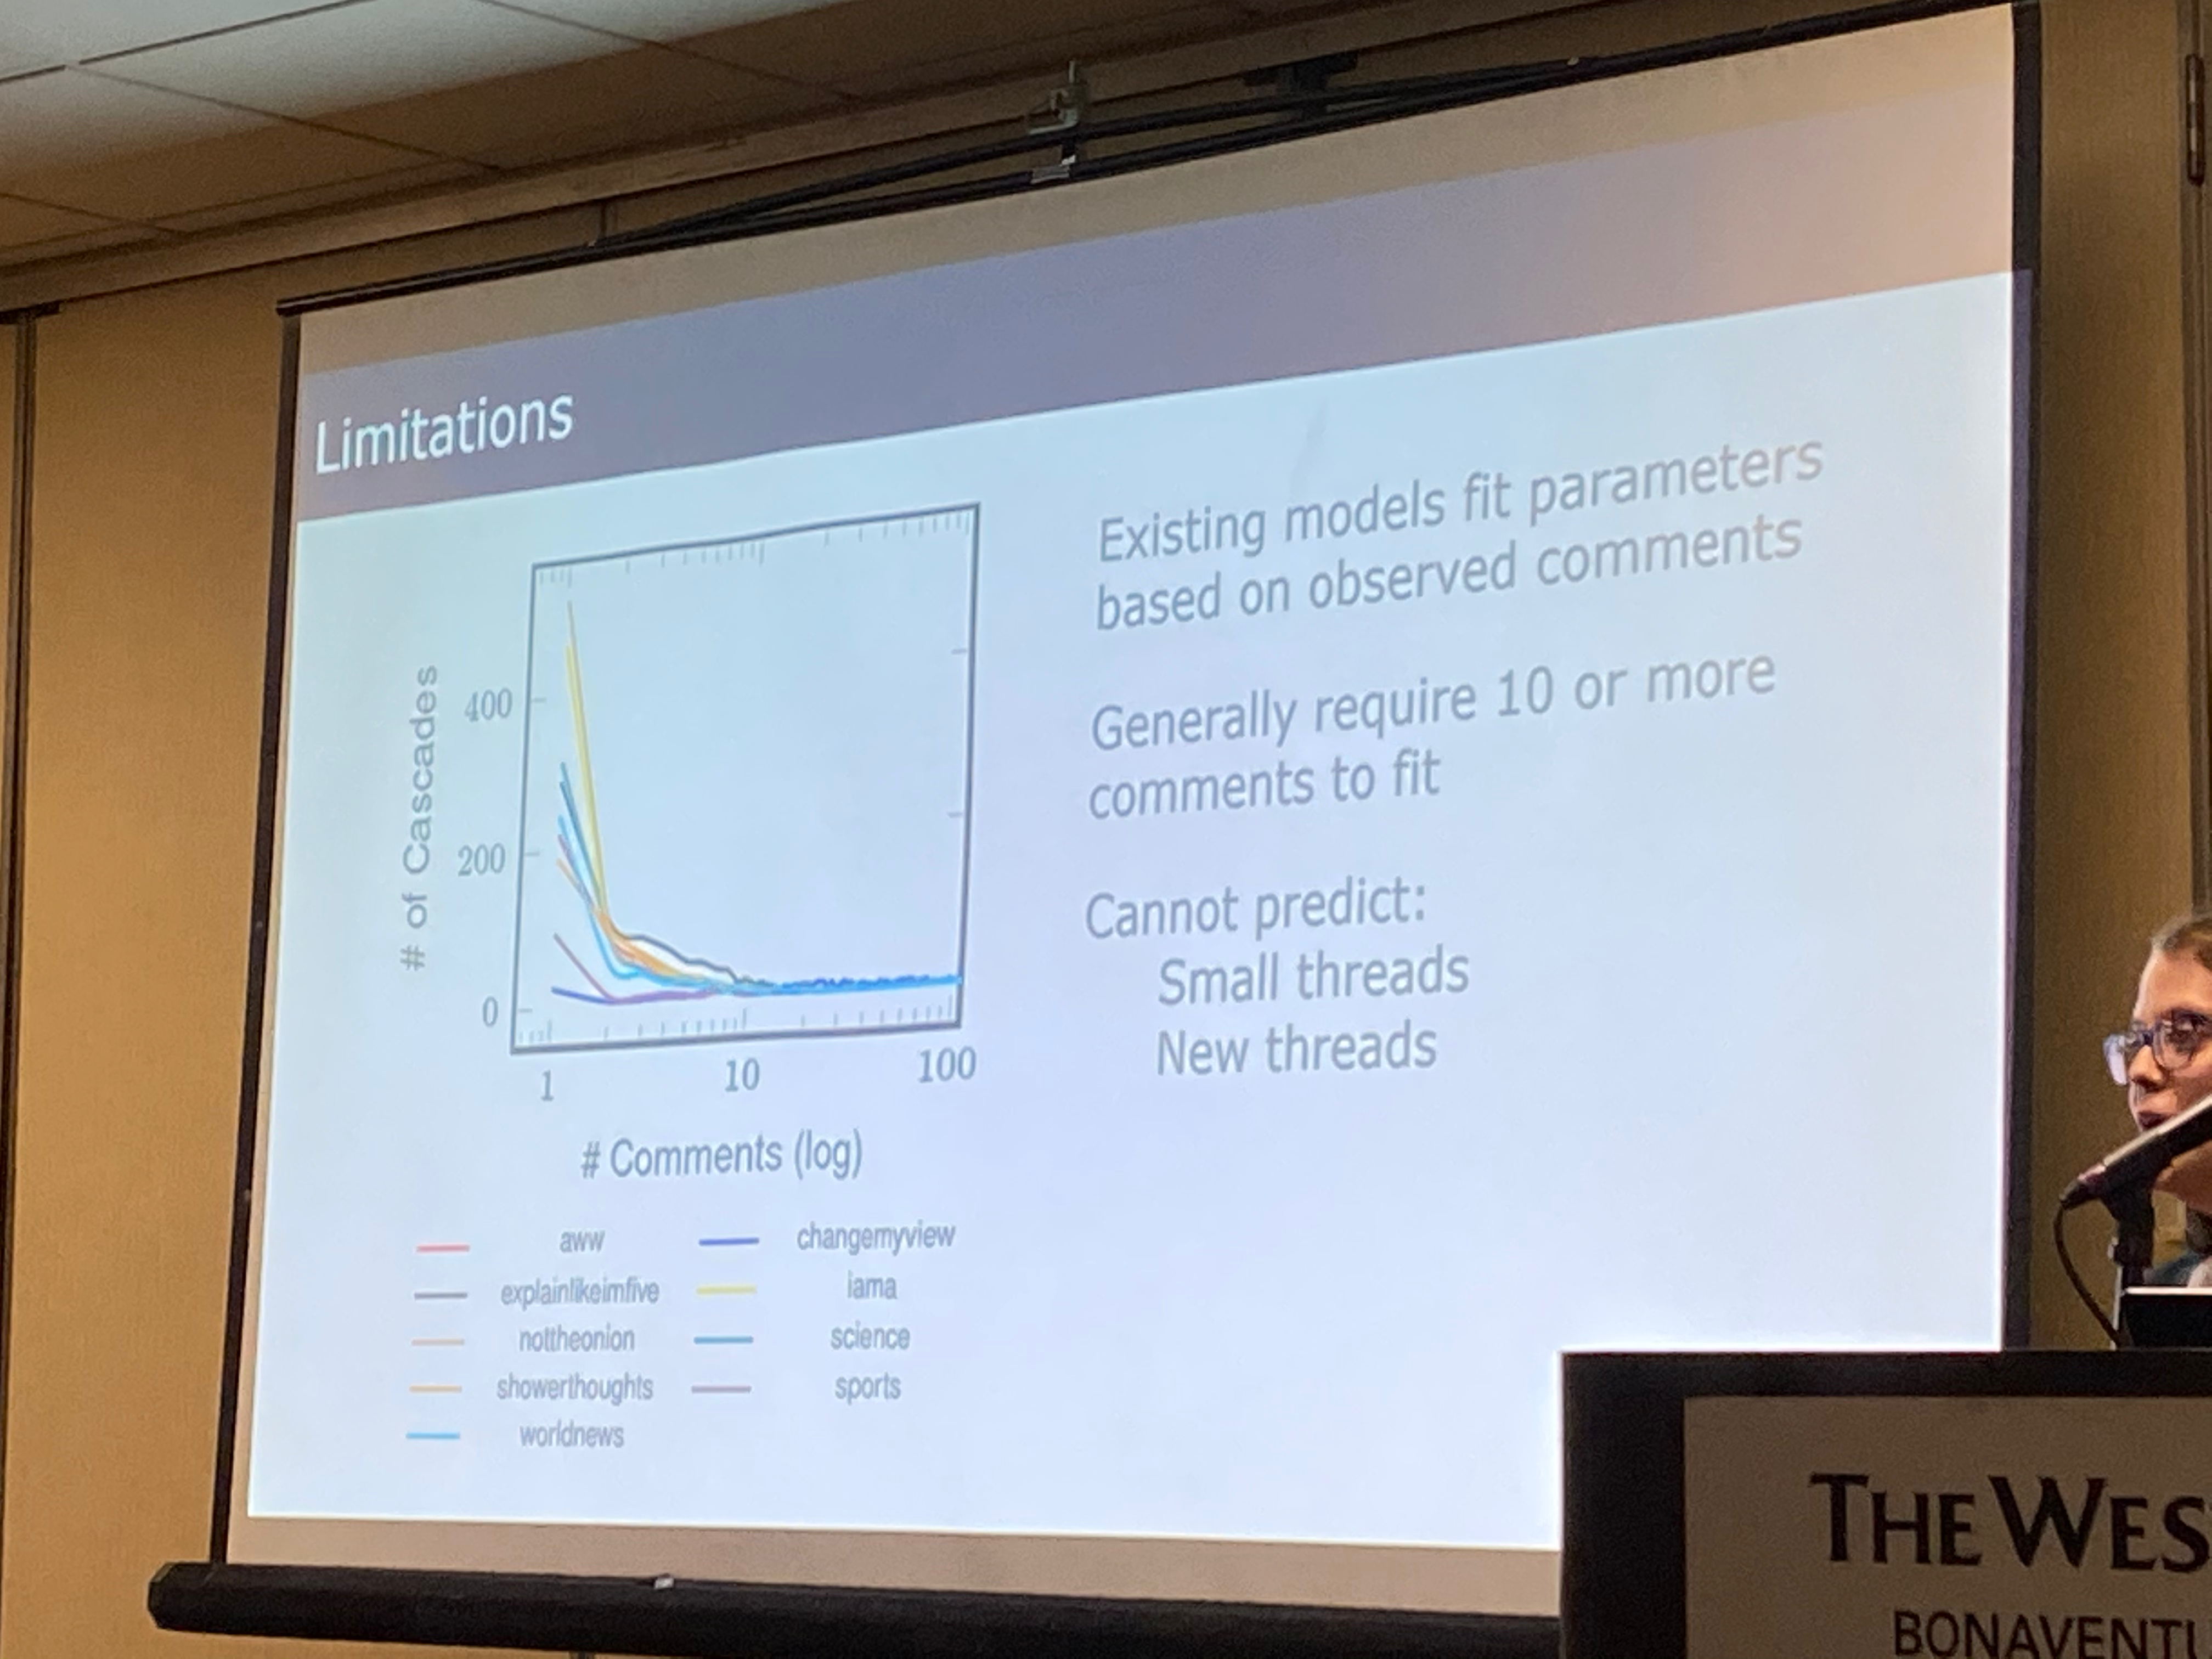
\includegraphics[width=120mm]{images/hawks_lim.png}
    \caption{Limitations of hawks process}
    \label{fig:my_label}
\end{figure}{}

\subsubsection{Improving Scalability of Parallel CNN Training by Adjusting Mini-Batch Size at Run-Time}

{\bf Challenge:} Training modern CNN models requires too much computing time which sometime hinders the practicality of new CNN models. Thus, parallel training is often adopted.

\begin{figure}
    \centering
    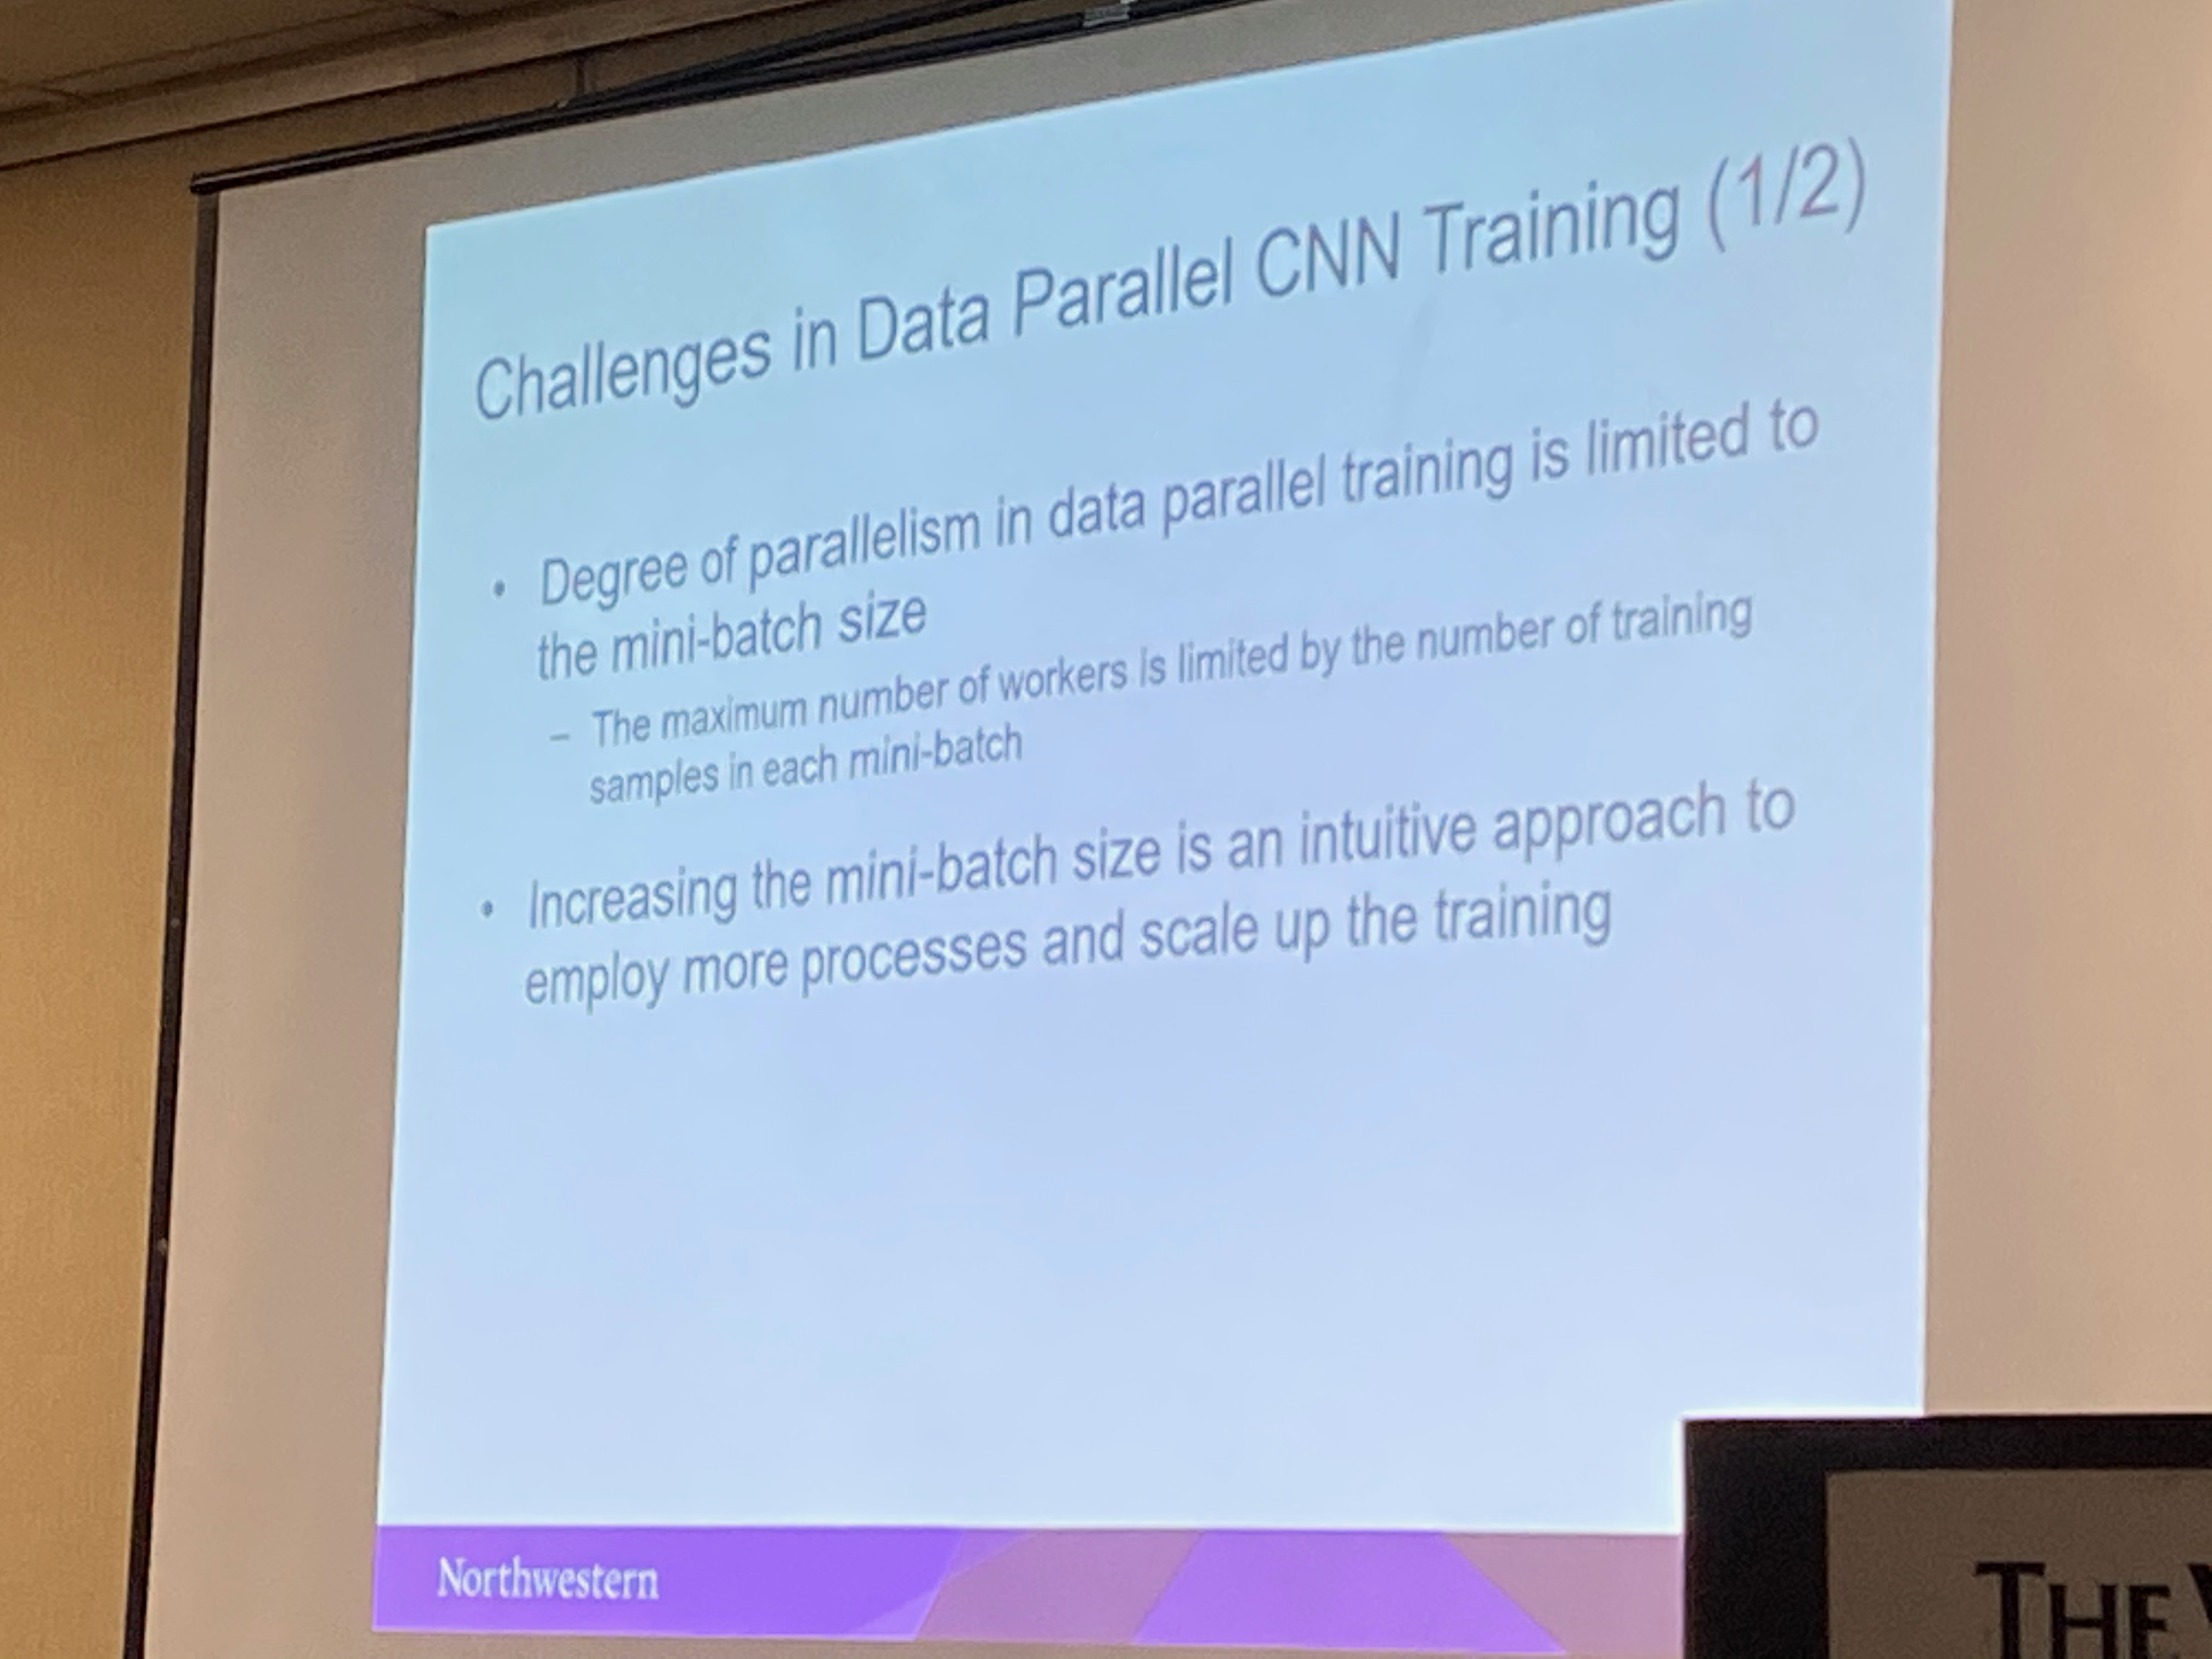
\includegraphics[width=120mm]{images/cnn_parallel.png}
    \caption{Data parallel CNN training}
    \label{fig:my_label}
\end{figure}{}

\begin{figure}
    \centering
    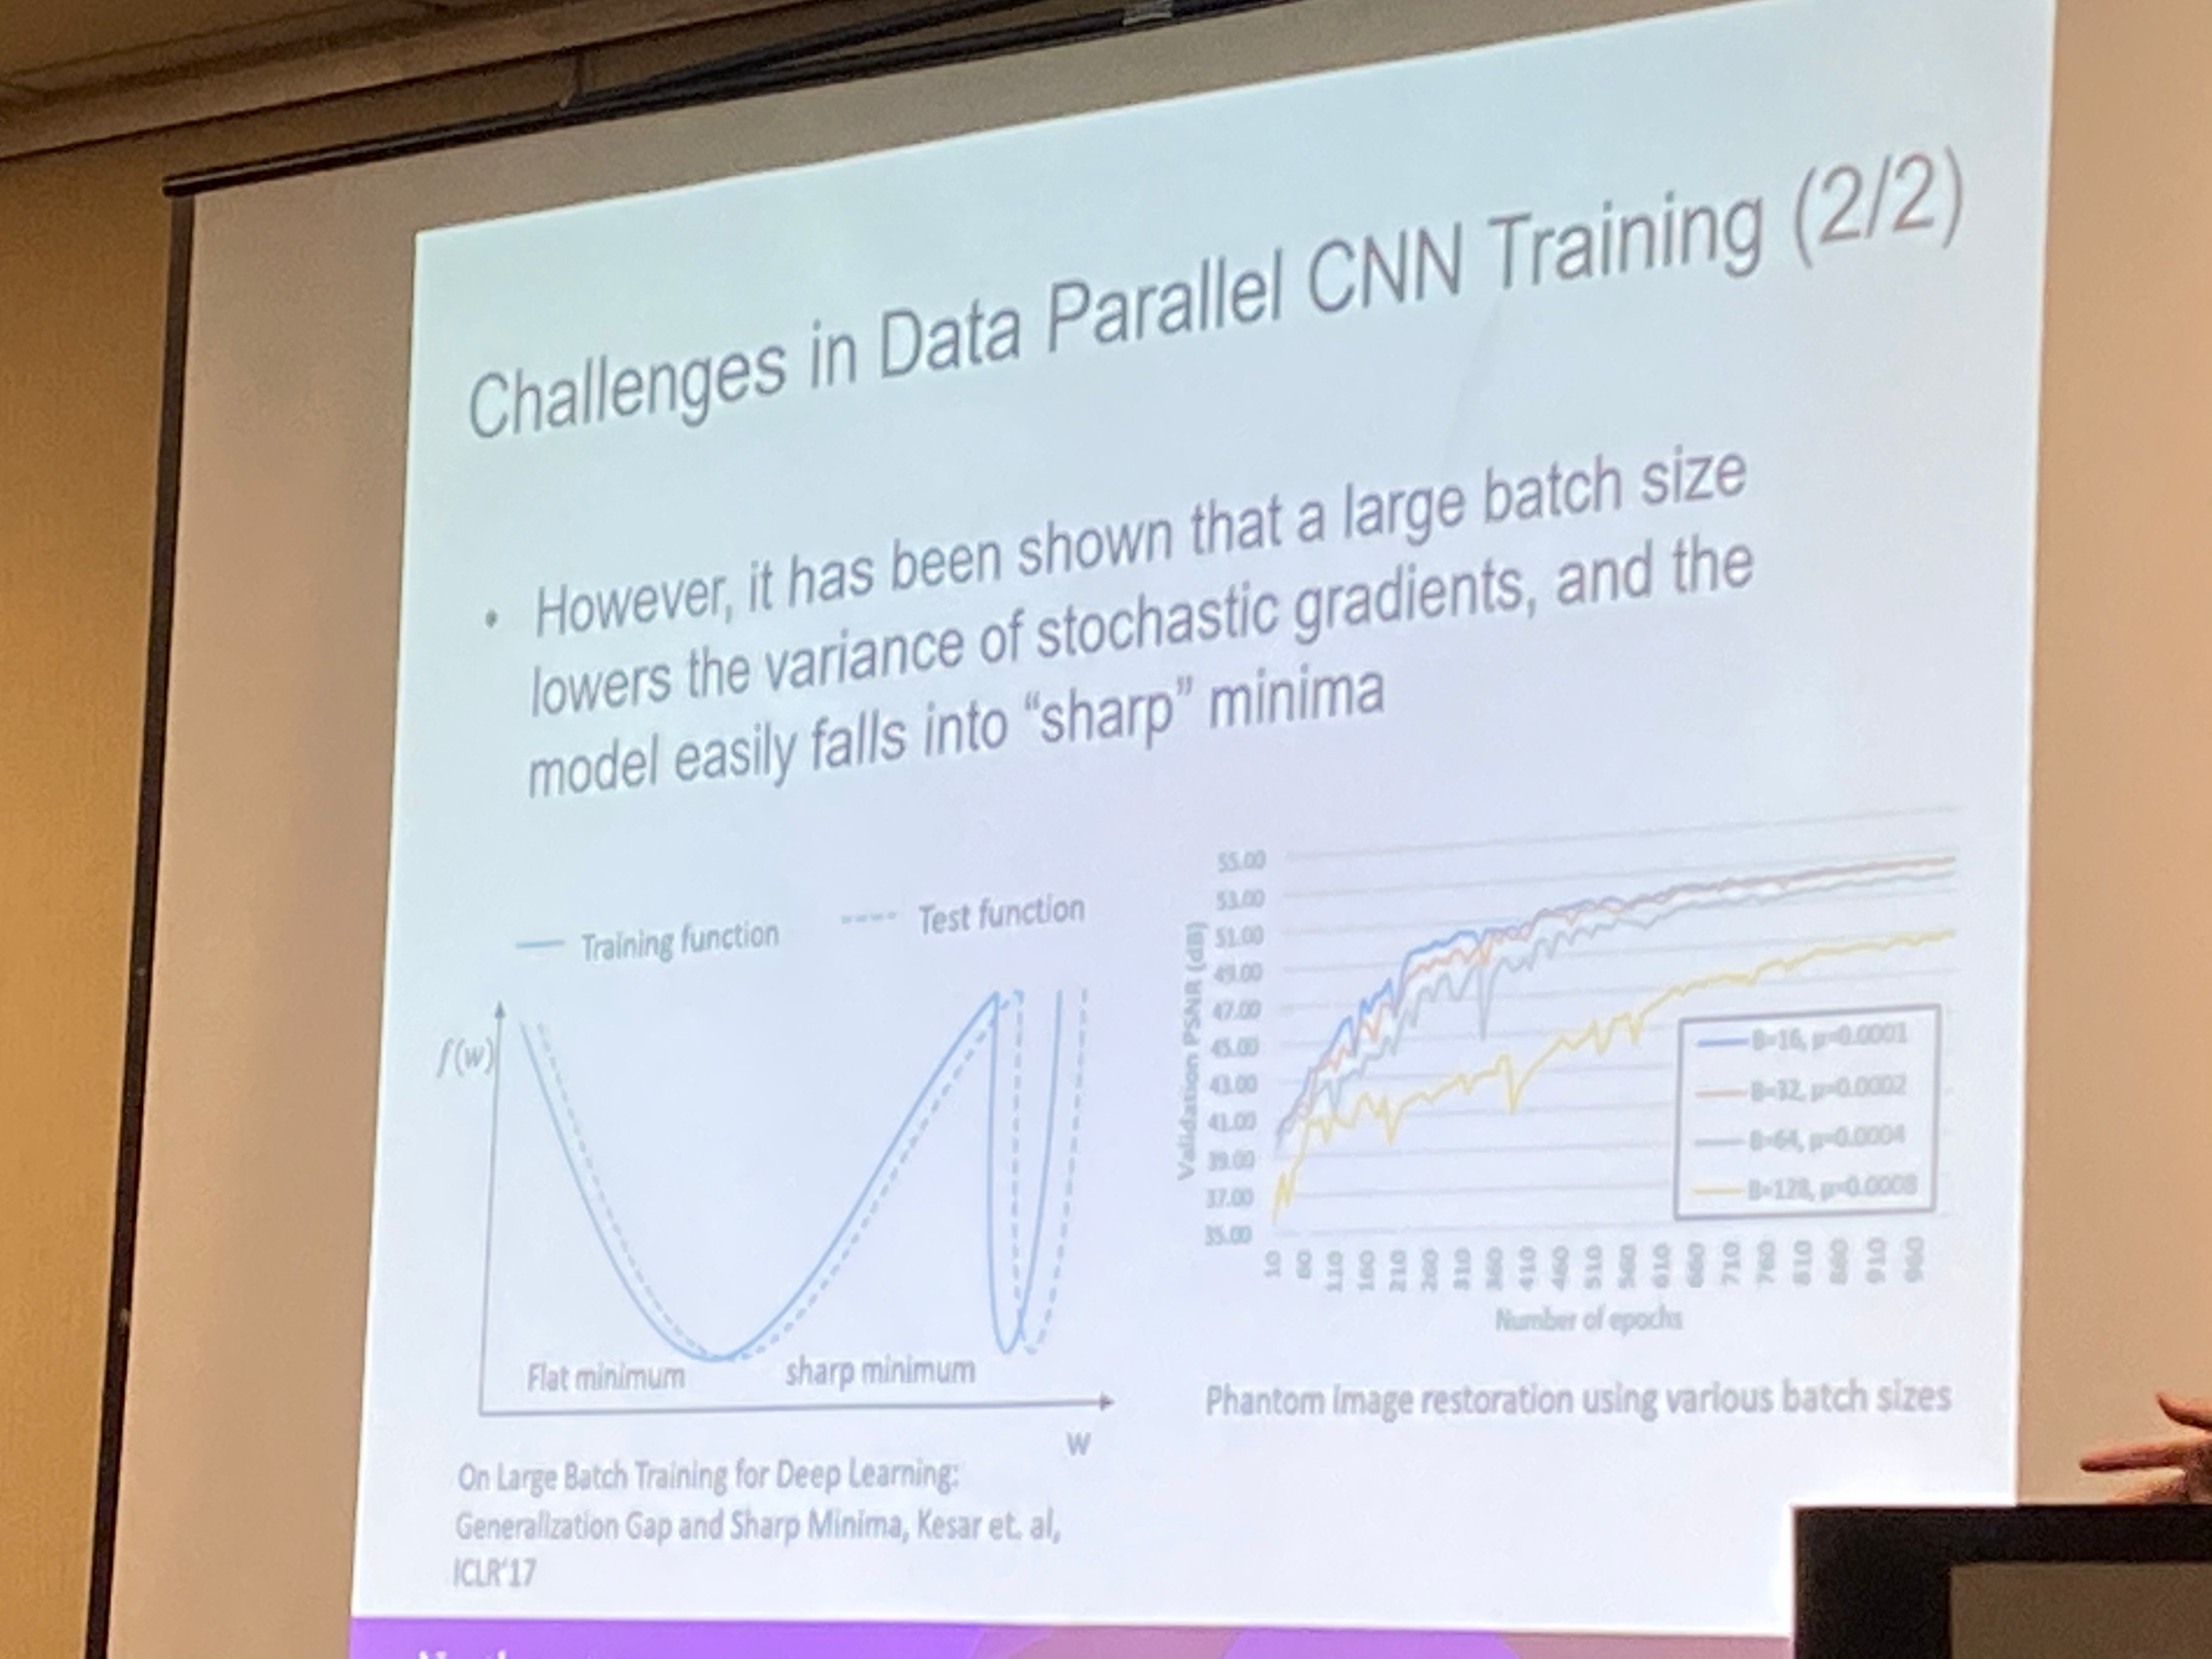
\includegraphics[width=120mm]{images/cnn_parallel_2.png}
    \caption{Data parallel CNN training2}
    \label{fig:my_label}
\end{figure}{}



\spacerule



% --- Bibliography ---
\newpage
\bibliographystyle{plainnat}
\bibliography{bigdata2019}

\end{document}